\documentclass[a4paper, 12pt]{scrreprt}

\usepackage[utf8]{inputenc}

\usepackage[T1]{fontenc}
\usepackage{listings}
\usepackage{float}
\usepackage{longtable}
\usepackage{graphicx}
\usepackage{hyperref}
\usepackage{textcomp}
\usepackage{caption}
\usepackage{parskip}
\usepackage[onehalfspacing]{setspace}
\usepackage{chngcntr}
\usepackage{acronym}
\usepackage{dirtree}
\usepackage{fancyhdr}
\usepackage[export]{adjustbox}
\usepackage[table,xcdraw,pdftex]{xcolor}
\usepackage{calc}
\usepackage{enumitem}
\usepackage{chngcntr}
\usepackage{jslistings}

\AtBeginDocument{\counterwithout{lstlisting}{chapter}}


\lstset{basicstyle=\normalsize\linespread{1}\ttfamily\small,
		breaklines=true,
		extendedchars=true,
		inputencoding=utf8,
		literate= 
			{ä}{{\"a}}1%
			{ö}{{\"o}}1%
			{ü}{{\"u}}1,%
}

\interfootnotelinepenalty=10000



\usepackage[
backend=biber,
sorting=none,
citestyle=authoryear,
natbib=true
]{biblatex}
\usepackage[ngerman]{babel}
\usepackage{enumitem}


\setlist[enumerate]{label*=\arabic*.}
\addbibresource{references.bib}
\hypersetup{
	colorlinks,
	linkcolor={black},
	citecolor={black},
	urlcolor={black}
}
\defbibfilter{bookInbook}{
	type=book or
	type=inbook
}
\graphicspath{ {./img/} }

\counterwithout{figure}{chapter}
\counterwithout{table}{chapter}

\newcommand\klammercite[1]{%
	(\citealt{#1})}

\parskip 1.75ex plus 0.5ex minus 0.5ex





\title{Synchronisierung von Daten in einer Offline-First Webanwendung mithilfe von CRDTs}
\subtitle{}
\author{Lennart Ploog}
\publishers{IS Medieninformatik\\ Fakultät 4\\ Hochschule Bremen}

\makeatletter
\let\inserttitle\@title
\makeatother

\begin{document}
\pagenumbering{gobble}
\begin{titlepage}

\centering

\includegraphics[width=0.30\textwidth]{hs_logo.png}
\par\vspace{1cm}
{\scshape\Large Hochschule Bremen \par}
{\scshape Fakultät 4 \\}
{\scshape Internationaler Studiengang Medieninformatik B.Sc. \par}
\vspace{1.5cm}
{\scshape\Large Bachelorthesis  \par}
\vspace{1.5cm}
{\LARGE\bfseries Synchronisierung von Daten in einer Offline-First Webanwendung mithilfe von CRDTs\par}
\vspace{1.5cm}

\newcolumntype{x}[1]{>{\raggedleft\arraybackslash\hspace{0pt}}p{#1}}
\begin{tabular}{x{6.5cm}p{6.5cm}}
	\rule{0mm}{5ex}\textbf{Autor:} & Lennart Ploog \\ 
	\rule{0mm}{5ex}\textbf{Matrikelnummer:} & 354556 \\ 
	\rule{0mm}{5ex}\textbf{Erstgutachter:} & Prof. Dr. Volker Paelke \\
	\rule{0mm}{5ex}\textbf{Zweitgutachter:} & Prof. Dr. Martin Hering-Bertram\\
	\rule{0mm}{5ex}\textbf{Abgabedatum:} & 28.08.2020\\
\end{tabular} 
\end{titlepage}
\newpage
\section*{Zusammenfassung}
Die Arbeit \enquote{\inserttitle} behandelt die Konzeption und Umsetzung einer Offline-First Webanwendung mit einer Datenstruktur auf Basis von konfliktfreien Replizierten Datentypen(CRDTs). Zuerst werden die Grundlagen vom Offline-First Prinzip und CRDTs erkundet. Dabei soll dem Leser vermittelt werden, wie und warum der Einsatz von CRDTs in Offline-First Applikationen hilfreich sein kann, denn die Themen stehen nicht zwangsläufig in Verbindung. Anschließend wird eine Webanwendung, welche auch offline vollständig nutzbar ist, als Prototyp konzipiert und umgesetzt. Die Datenstruktur wird mithilfe von CRDTs so umgesetzt, dass ein konfliktfreies Synchronisieren von Daten mit einem Server möglich ist, auch wenn Änderungen offline erfolgt sind. Nach der Fertigstellung des Prototypen folgt eine Evaluation der entwickelten Anwendung und ihrer Funktionalitäten. Abgeschlossen wird die Arbeit mit dem Fazit, in welchem zusammengefasst wird welche Erkenntnisse über den Einsatz von CRDTs in Offline-First Anwendungen gewonnen werden konnten.

\section*{Abstract}
The bachelors thesis \enquote{Data Synchronization In A Offline-First Web Application Using CRDTs} discusses the design and implementation of an offline-first web application with a data structure based on conflict-free replicated data types(CRDTs). First, the basics of the offline-first principle and CRDTs are explored. Because the topics are not necessarily related, the reader is given an explanation how and why the use of CRDTs in offline-first applications can be helpful. Subsequently, a web application, which is fully usable offline, is designed and implemented as a prototype. With the help of CRDTs, the data structure is implemented to allow conflict-free synchronization of it's data with a server, even if changes have been made offline. After completion of the prototype an evaluation of the developed application and its functionalities is conducted. The thesis is concluded with a summary of the gained knowledge on the use of CRDTs in offline First applications.
\newpage

\pagestyle{fancy}
\cfoot{\thepage}
\lhead[\leftmark]{}
\rhead[]{\leftmark}

\tableofcontents
\newpage
\section*{Abkürzungsverzeichnis}
	\begin{acronym}[Bash]
		\acro{CRDT}{Conflict-free replicated data type}
		\acrodefplural{CRDT}{Conflict-free replicated data types}
		\acro{PWA}{Progressive Web-App}
		\acrodefplural{PWA}{Progressive Web-Apps}
		\acro{SC}{Strong Consistency}
		\acro{SEC}{Strong Eventual Consistency}
		\acro{EC}{Eventual Consistency}
		\acro{P2P}{Peer To Peer}
		\acro{HLC}{Hybrid Logical Clock}
		\acro{JSON}{JavaScript Object Notation}
		\acro{HTTP}{Hypertext Transfer Protocol}
		\acro{HTTPS}{Hypertext Transfer Protocol Secure}
		\acro{LWW}{Last-Write-Wins}
		\acro{LWW-Register}{Last-Write-Wins Register}
		\acro{G-Set}{Grow-Only Set}
		\acro{CORS}{Cross-Origin Resource Sharing}
		\acro{BaaS}{Backend as a Service}
	\end{acronym}

\newpage
\pagenumbering{arabic}
\chapter{Einleitung}\label{sec:Einleitung}
\section{Problemfeld}\label{sec:Problemfeld}

Ob auf Reisen, im Supermarkt oder im Fahrstuhl -- Situationen, in denen mobile Endgeräte keine stabile Internetverbindung haben, kommen im Alltag häufiger vor als gewünscht. In vielen Entwicklungsländern und auch in ländlichen Gegenden entwickelter Industriestaaten fehlt dafür gar die komplette Infrastruktur. Im Laufe der letzten Jahre eröffneten Innovationen im Bereich der Browser-Technologien, allen voran der Service-Worker, neue Möglichkeiten für die Webentwicklung, insbesondere für sogenannte Offline-First Anwendungen. Als Offline-First Applikationen werden Webanwendungen bezeichnet, die ihre Funktionalität so weit es geht behalten, wenn die Verbindung zum Internet getrennt ist.

Eine der Kernherausforderungen der Entwicklung von Offline-First Applikationen ist die Synchronisation von Daten. Werden offline Änderungen vorgenommen, sollen diese nicht verloren gehen. Hat sich der Zustand der Applikation, beispielsweise durch Modifikationen eines anderen Nutzers, in der Zwischenzeit jedoch geändert, müssen beide Änderungen zusammengebracht, also synchronisiert werden. Der Prozess der Synchronisation ist oft aufwendig, denn zum Einen muss ermittelt werden, wo sich beide Replikationen unterscheiden und zum Anderen muss vermieden werden, dass die Änderungen sich in die Quere kommen. 

Gängige Lösungen zu einer solchen Zusammenführung von Daten umfassen die Nutzung bestimmter Datenbanken-Technologien. Dazu gehören Datenbanken mit implementierter Synchronisation wie CloudDB oder auch \ac{BaaS} Produkte wie Firebase oder IBM Cloudant, welche ebenfalls eine solche Funktionalität anbieten. Um zu vermeiden, die Applikation mit suboptimalen Datenbanken-Technologien umsetzen zu müssen, verzichten viele Applikationen bei Konflikten auf eine Synchronisation und einer der beiden Nutzer verliert seine vollbrachte Arbeit.

\section{Ziel der Arbeit} 

Ziel dieser Arbeit ist es, eine Lösung zur Synchronisation von Daten in Offline-First Anwendungen mit Hilfe von konfliktfreien replizierten Datentypen (\acp{CRDT}) umzusetzen. Der Einsatz von \acp{CRDT} ermöglicht, dass Daten in einem verteilten System in beliebiger Reihenfolge ausgetauscht werden können und dennoch zum gleichen Zustand aller Replikationen führen. Durch die Implementierung einer Datenstruktur, welche auf \acp{CRDT} aufbaut, kann der Prozess der Synchronisierung somit vermieden werden. Diese Lösung soll unabhängig von der gewählten Datenbank sein.

So ergeben sich folgende Forschungsfragen:

\begin{itemize}
	\item Wie können \acp{CRDT} in Offline-First Applikationen verwendet werden?
	\item Welche \acp{CRDT} bieten sich zur Umsetzung von Offline-First Applikationen an und wie werden diese in die Datenbanken (Client und Server) implementiert?
	\item Welche Vor- und Nachteile bietet die Nutzung von \acp{CRDT} im Vergleich zu anderen Optionen zur Synchronisierung von Daten in Offline-First Applikationen?
\end{itemize}

\section{Vorgehen}
Es gibt verschiedene Möglichkeiten, wie \acp{CRDT} in Webapplikationen eingesetzt werden können. Bevor die Implementation der Datenstruktur im hier entwickelten Prototypen beginnen kann, muss ermittelt werden, welche \acp{CRDT} sich am besten für die Daten des Prototypen eignen. Um dies herauszufinden, eignet sich die Recherche in den im Abschnitt Verwandte Arbeiten erwähnten Publikationen. Darüber hinaus lohnt es sich an dieser Stelle auch in Erfahrung zu bringen, welche \acp{CRDT} bis heute in fertigen Applikationen verwendet wurden. Auch Literatur zum Austausch von Daten in Applikationen zu kollaborativem Editieren in \ac{P2P} Netzwerken bietet sich zur Recherche an, denn in diesen Bereichen sind \acp{CRDT} schon weiter verbreitet als in anderen Anwendungsgebieten.

Damit der Prototyp als praxisnahes Beispiel dienen kann, sollte auch der Stand der Technik im Themenbereich der Offline-First Anwendungen ermittelt werden. Um einzuordnen, auf welcher Ebene der Architektur der Applikation sich die umzusetzende Funktionalität zur Zusammenführung der Daten am besten einbauen lässt, lohnt sich auch ein Blick auf bestehende Lösungen, welche die Synchronisation nicht direkt auf der Datenbankebene durchführen, sondern zwischen Applikation und Datenbank.

\chapter{Grundlagen}
Dieses Kapitel erläutert die Grundlagen, Ideen und Konzepte, auf welchen Offline-First Applikationen und \acp{CRDT} aufbauen. 

\section{Verwandte Arbeiten}
\label{sec:VerwandteArbeiten}

\acp{CRDT} sind aus der Forschung an Datenstrukturen für kollaboratives Editieren entstanden. \citet{InproceedingsCRDTOriginal} formulieren die theoretischen Grundlagen von \acp{CRDT}, um \ac{SEC} in großen verteilten Systemen zu garantieren. \ac{SEC} erweitert den bis dahin verbreiteten Ansatz der \ac{EC}. Während EC nur garantiert, dass sämtliche Updates schlussendlich alle Replizierungen der Datenbank erreichen, garantiert SEC zusätzlich, dass Updates unabhängig von Reihenfolge und Zeitpunkt immer zum gleichen Zustand der Replizierungen führen.

Seitdem hat sich die Verwendung von \acp{CRDT} in verschiedenen Bereichen der Webentwicklung verbreitet. \citet{ArticleCRDTJSON} entwerfen eine Bibliothek CRDT konformer \ac{JSON} Datenstrukturen, genannt \enquote{automerge}, die beliebig verschachtelte Listen und Maps unterstützt. Mit \enquote{Hypermerge} entstand auch eine spezielle Version für Peer-to-Peer Netzwerke. Eine weitere Bibliothek, die vorgefertigte \acp{CRDT} bereitstellt ist yjs\autocite{inproceedingsYjs}. Einen wichtigen Anhaltspunkt für die Nutzung in Offline-First Applikationen bietet der Vortrag \enquote{\acp{CRDT} for Mortals} \autocite{OnlineCrdtsForMortals}, in welchem über den Einsatz von \acp{CRDT} im Client-Server Modell gesprochen wird.  

Mit Woot \klammercite{InproceedingsCRDTWoot}, Logoot \klammercite{InproceedingsCRDTLogoot} und LSEQ \klammercite{InproceedingsCRDTLSEQ} sind bereits \acp{CRDT} speziell für den Bereich des kollaborativen Editierens entwickelt worden. 

Der Anzahl an Quellen und Ressourcen rund um \acp{CRDT} mangelt es weder an theoretischen noch an praktischen Beispielen. Während einige Arbeiten die Nutzung von \acp{CRDT} für Offlinefunktionalität empfehlen und die Umgebung von Offline-First Applikationen sehr den verteilten Netzwerken ähnelt, für die \acp{CRDT} konzipiert sind, sind dem Autoren keine wissenschaftlichen Arbeiten über den konkreten Einsatz von \acp{CRDT} in Offline-First Webanwendungen bekannt. Ziel dieser Arbeit ist es deshalb, die umfangreich erforschten Grundlagen zum Einsatz von \acp{CRDT} in einer Offline-First Webanwendung umzusetzen und zu ermitteln, wie dies bei der Bewältigung der Herausforderungen dieser Umgebung, helfen kann.

\section{Definition: Offline-First}\label{sec:DefinitionOfflineFirst}
Als Offline-First wird ein Vorgehen bezeichnet, bei welchem eine Applikation den Fall der unterbrochenen Internetverbindung nicht als Ausnahme, sondern als Standard ansieht \autocite{OnlineGoogleProgressiveWebApps}. Teilweise wird der Begriff auch anders interpretiert, im Rahmen dieser Arbeit sei Offline-First jedoch unter folgenden Kriterien zu verstehen: Die Applikation geht davon aus, dass die Verbindung mit dem Internet nach dem ersten Laden der Seite stets unterbrochen werden kann. Dies gilt auch im Falle von Verbindungsproblemen, welche nicht vom Endgerät des Nutzers als solche erkannt werden, z.B. wenn das Endgerät mit dem Internet verbunden ist, aber die Route zur Website an anderer Stelle unterbrochen ist. Sämtliche Use-Cases werden so geplant, dass dem Nutzer auch offline so viele Funktionalitäten wie möglich zur Verfügung stehen \autocite{ArticleDesigningOfflineFirst}. 



\section{Service Worker}
\label{sec:serviceworker}

Ein Service Worker ist ein sogenannter Web Worker. Web Worker sind Skripte, die unabhängig von anderen Skripts, welche auf Interaktionen mit der Benutzeroberfläche reagieren, im Hintergrund der Webanwendung laufen \autocite{OnlineHTTPWorker}.

In traditionellen Webanwendungen werden alle benötigten Dateien, Markups, Skripte und Assets über \ac{HTTP}-Requests an den Server angefordert. Der Service Worker ist ein event-basiertes Skript, welches als Proxy zwischen Client und Server agiert. Damit diese Tatsache kein Sicherheitsrisiko darstellt, funktionieren Service Worker nur, wenn die Applikation \ac{HTTPS} nutzt. Requests, welche üblicherweise direkt an den Server gehen würden, werden erst vom Service Worker verarbeitet. Entwickler können gezielt entscheiden, welche Netzwerk-Requests auf welche Art und Weise verarbeitet werden sollen. Mithilfe dieser Funktionalität können Entwickler sogenannte Caching-Strategien für den Service Worker implementieren, womit das Verbindungsverhalten der Applikation festgelegt werden kann \autocite{OnlineServiceWorkersAnIntroduction}. Dies ist eine für Offline-First Applikationen essenzielle Funktionalität, denn so kann garantiert werden, dass die Applikation auch ohne Internetverbindung funktionsfähig ist. 

\section{Caching}
In dieser Sektion werden einige grundlegende Caching-Strategien beschrieben, mit Beispielen, für welche Art von Requests sie sich eignen könnten.

\subsubsection{\enquote{Erst Netzwerk, dann Cache}}
Abbildung \ref{fig:cachingNetworkFirst} beschreibt einen Request, den der Service Worker zuerst über das Netzwerk delegiert. Falls die Kommunikation mit dem Internet unterbrochen ist, beispielsweise wenn der Nutzer offline ist, leitet der Service Worker den Request an den Cache weiter. Diese Methode eignet sich für Requests, bei denen aktuelle Daten bevorzugt sind, dem Nutzer aber eine ältere Version zur Verfügung gestellt werden soll, wenn die Internetverbindung unterbrochen ist.

\begin{figure}[H]
	\centering
	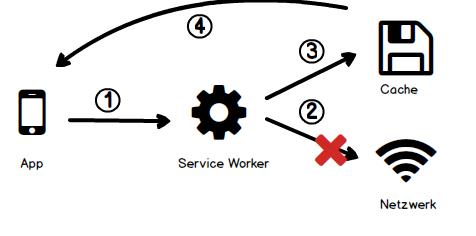
\includegraphics[width=0.75\textwidth]{networkfirst.png}
	\caption{Caching-Strategie: \enquote{Erst Netzwerk, dann Cache}}
	\label{fig:cachingNetworkFirst}
\end{figure}



\subsubsection{\enquote{Erst Cache, dann Netzwerk}}
\label{sec:cachedannnetzwerk}
Wie Abbildung \ref{fig:cachingCacheFirst} zeigt, wird der Request hier zuerst an den Cache weitergeleitet. Befindet sich die angefragte Datei nicht im Cache, wird die Anfrage als \ac{HTTP}-Request an den Server weitergeleitet. Dies ist die bevorzugte Strategie für die meisten Requests in Offline-First Anwendungen.\autocite[Kapitel 05]{BookBuildingPWAs}.

\begin{figure}[H]
	\centering
	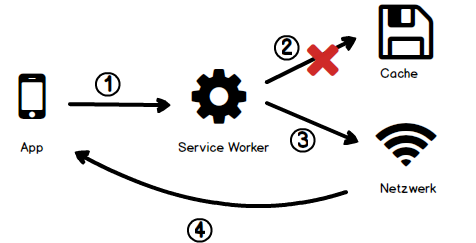
\includegraphics[width=0.75\textwidth]{cachefirst.png}
	\caption{Caching-Strategie: \enquote{Erst Cache, dann Netzwerk}}
	\label{fig:cachingCacheFirst}
\end{figure}

\subsubsection{\enquote{Nur Netzwerk}}
Für Aufgaben, die nur online zu erfüllen sind, eignet sich die in Abbildung \ref{fig:cachingNetworkOnly} bezeichnete Strategie. Hier leitet der Service Worker den Request nur an das Netzwerk und nie an den Cache weiter. Offline-First Applikationen sollten so konzipiert sein, dass diese Art Requests im Falle einer unterbrochenen Internetverbindung nachgeholt werden können, wenn der Nutzer wieder online ist.

\begin{figure}[H]
	\centering
	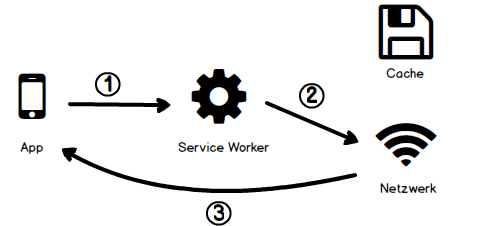
\includegraphics[width=0.75\textwidth]{networkonly.png}
	\caption{Caching-Strategie: \enquote{Nur Netzwerk}}
	\label{fig:cachingNetworkOnly}
\end{figure}

\subsubsection{\enquote{Nur Cache}}
Abbildung \ref{fig:cachingCacheOnly} zeigt, wie die angefragte Ressource nur im Cache abgefragt wird. Diese Strategie ist nur dann sinnvoll, wenn die betroffenen Daten in einem vorherigen Schritt, beispielsweise beim Installieren des Service Workers, mit gecached wurden.

\begin{figure}[H]
	\centering
	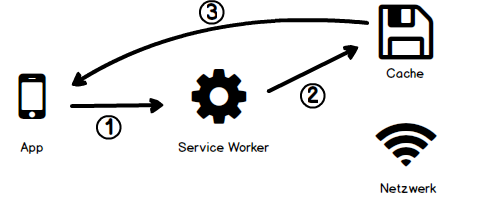
\includegraphics[width=0.75\textwidth]{cacheonly.png}
	\caption{Caching-Strategie: \enquote{Nur Cache}}
	\label{fig:cachingCacheOnly}
\end{figure}

\section{Offline First Applikationen als verteilte Systeme}\label{sec:OfflineFirstVerteiteSysteme}
\citet{ArticleDistributedSystems} beschreiben verteilte Systeme wie folgt: \enquote{Ein verteiltes System ist eine Sammlung von autonomen Rechenelementen, die den Benutzern als ein einziges kohärentes System erscheint.}

Die folgende Liste zeigt die Charakteristika von verteilten Systemen, zusammengefasst nach \citet{BookDistributedSystemsDefinition}.

\begin{description}
\item[Eigenständige Computer] In einem verteilten System sind mehrere eigenständige Computer zu einem System verbunden. Diese können sich sowohl in der Hardware als auch in der Funktionsweise unterscheiden. 
\item[Singuläres Erscheinungsbild] Für den Nutzer sind die Unterschiede zwischen den einzelnen Computern im System unersichtlich. Er nimmt die verteilten Computer als ein einzelnes System wahr. 
\item[Konsistente und einheitliche Interaktion]
	Eine Konsequenz aus dem singulären Erscheinen ist, dass die Interaktion des Nutzers mit dem System immer gleich sein sollte, unabhängig davon, mit welcher Schnittstelle des Systems er tatsächlich interagiert. 
\item[Kontinuierliche Verfügbarkeit]
	Das System soll dem Nutzer kontinuierlich zur Verfügung stehen, auch wenn einzelne Teile des Systems vorübergehend ausgefallen oder nicht erreichbar sind.
\end{description}
\label{tab:charakteristikaDistributedSystem}

%TODO satz einfügen Kleppnmann vortrag.
Die folgende Liste zeigt, dass funktionsfähige Offline-First Applikationen die gleichen Charakteristika aufweisen und fasst zusammen, welche Rolle diese Merkmale in der Applikation spielen.

\begin{description}		
\item[Eigenständige Computer] Der Server und verschiedene Endgeräte bilden ein System. Sobald ein Endgerät die Applikation zwischenspeichert, ist sie als eigenständiger Computer im System aktiv. Als Endgerät qualifiziert sich jedes Gerät, welches einen kompatiblen Browser betreibt, weshalb die Endgeräte auch untereinander über unterschiedlichste Hardware verfügen können.
\item[Singuläres Erscheinungsbild]Die Kernfunktionalität von Offline-First Applikationen ist die Offlinefunktionalität \autocite{OnlineGoogleOfflineFirst}. Offline interagiert der Nutzer nur mit seinem Endgerät, online werden die Daten gleich an den Server geschickt. Diese Unterschiede sind für den Nutzer jedoch nicht von Belang. \item[Konsistente und einheitliche Interaktion]
Unabhängig davon, welches Endgerät der Nutzer verwendet, sollen ihm früher oder später die Änderungen aller im System aktiven Geräte angezeigt werden. Der Nutzer muss sich zu keinem Zeitpunkt Gedanken darüber machen, aus welchen Computern das System besteht.
\item[Kontinuierliche Verfügbarkeit]
Ein weiterer Aspekt, welcher sich aus der verbindlichen Offlinefunktionalität ergibt, ist die kontinuierliche Verfügbarkeit. Der Nutzer kann seine Arbeit auch fortführen, wenn der Server nicht erreichbar ist. Durch SEC landen diese Änderungen früher oder später im System, wodurch die getrennte Verbindung zum Server keine Auswirkungen auf dessen Funktionsumfang hat. 
\end{description}
\label{tab:charakteristikaOfflineFirst}

Daraus ergibt sich, dass es sich bei Offline-First Webanwendungen um verteilte Systeme handelt. Diese Erkenntnis kann dabei helfen, Probleme von Offline-First Applikationen zu lösen. Bei Offline-First handelt es sich um ein relativ junges Konzept. Obwohl Progressive Web Apps mittlerweile häufig im Netz anzutreffen sind, erfüllt deren Offlinefunktionalität selten Offline-First Kriterien. Für Probleme wie die in Abschnitt \ref{sec:Problemfeld} beschriebene Synchronisation von Daten gibt es deshalb wenige beschriebene Lösungsansätze oder konkrete wissenschaftliche Arbeiten (vgl. Sektion \ref{sec:VerwandteArbeiten}). Mit verteilten Systemen hingegen beschäftigt sich die Informatik bereits seit den 70er Jahren \autocite{Andrews1999FoundationsOM}. Lösungen, welche für die Herausforderungen von verteilten Systemen entwickelt wurden, kommen also auch für Offline-First Webapplikationen in Frage. Eine dieser Lösungen ist die Nutzung von optimistischen Replikationsverfahren. 

\section{Replikation}

Eine der wichtigsten Grundlagen verteilter Systeme ist die Replikation von Daten. Datenreplikation beschreibt das Verwalten mehrerer Datenspeicher, genannt Replikationen. Diese Replikationen halten die gleichen Daten, befinden sich jedoch auf unterschiedlichen Computern \autocite[S.42]{ArticleOptimisticReplication}. \citet{BookDistributedSystemsConceptsAndDesign} nennen drei Aspekte, zu denen Replikation in verteilten Systemen entscheidend beiträgt: Performancesteigerung, erhöhte Verfügbarkeit und Fehlertoleranz. Somit trägt diese Technik entscheidend dazu bei, sowohl kontinuierliche Verfügbarkeit als auch konsistente Interaktion, beschrieben in \ref{tab:charakteristikaDistributedSystem}, zu garantieren. Vom aus dem Netz nicht mehr wegzudenkenden Caching bis hin zu aufwendigeren Aufgaben wie Load-Balancing oder der Verarbeitung von DNS-Requests bietet das Internet zahlreiche Anwendungsfelder, in denen Replikation angewendet wird. 

\subsection{Pessimistische Replikation: Strong Consistency}

Traditionelle Strategien, um die Replikationen auf dem selben Stand zu halten, folgen dem Modell der \ac{SC}. \ac{SC} setzt voraus, dass alle Replikationen stets identisch sind, als gäbe es konstant nur eine singuläre Kopie der Daten. Wenn ein Update auf einer Replikation erfolgt, muss es direkt auf allen weiteren Replikationen übernommen werden. 

Es gibt ein weites Spektrum an Lösungen, um \ac{SC} zu gewährleisten. Diese reichen von {Update-Everywhere} Systemen, die einzelne Änderungen sofort auf allen Replikationen speichern \autocite{ThesisUpdateEverywhere} bis zu \enquote{primary copy} Lösungen \autocite[S.14]{BookPrimaryReplica}, welche Änderungen von einem primären Datenspeicher auf alle weiteren Replikationen verteilen. Gemeinsam haben diese Algorithmen die Tatsache, dass sie keinen Zugriff auf Replikationen gewähren, welche nicht auf dem aktuellsten Stand sind \autocite[S.43]{ArticleOptimisticReplication}. Für Offline-First Anwendungen kommt diese Art der Replikation nicht in Frage. Die Anforderung, dass die Verbindung zum Netzwerk stets unterbrochen sein kann (vgl. \ref{sec:DefinitionOfflineFirst}), ist mit diesem Prinzip nicht vereinbar. Sobald eine Replikation vom Netzwerk getrennt ist, ist es unmöglich zu garantieren, dass sie auf dem aktuellsten Stand ist.


\subsection{Optimistische Replikation: Eventual Consistency}

Die optimistische Replikation, auch genannt \acf{EC}, ist ein alternatives Modell der Datenreplikation, welches den Replikationen erlaubt, voneinander abzuweichen.

Die Implementierung von optimistischer Replikation bietet sich somit als Lösung für Systeme an, welche besonderen Wert auf kontinuierliche Verfügbarkeit legen, wie Offline-First Applikationen (vgl. Sektion \ref{sec:OfflineFirstVerteiteSysteme}). 

Bei der Verwendung von optimistischer Replikation sind Änderungen an Replikationen jederzeit gestattet, auch wenn diese nicht auf dem aktuellsten Stand sind, oder keine Verbindung zum Netzwerk haben. Nimmt der Nutzer eine Änderung vor, so wird diese auf seiner Replikation sofort umgesetzt. Im Hintergrund wartet die Applikation nun darauf, diese Änderung an die restlichen Computer des verteilten Systems weiterzugeben sowie selbst Änderungen entgegenzunehmen und zu verarbeiten \autocite[S.46]{ArticleOptimisticReplication}. Ziel ist es, wie beim Modell der Strong Consistency, Einheitlichkeit unter den Replikationen herzustellen. Das Modell der \ac{EC} setzt jedoch nicht voraus, dass diese Einheitlichkeit sofort erfolgen muss, sondern nur zu einem beliebigen späteren Zeitpunkt. 

Da die Computer im System parallel Änderungen vornehmen können, kann es vorkommen, dass mehrere Replikationen das gleiche Datenobjekt modifizieren. Im Allgemeinen werden die Modifikationen zu unterschiedlichen Ergebnissen führen. Ist dies der Fall, spricht man von einem Konflikt. Das Ziel, Konvergenz zwischen den Replikationen zu erlangen, kann nur erreicht werden, wenn aus allen im Konflikt stehenden Änderungen eine einheitliche Lösung entsteht.

Deshalb muss ein System, welches \ac{EC} implementiert, die Funktionalität aufweisen, Konflikte zu beheben. Problematisch dabei ist, dass die Replikationen nicht auf dem gleichen Stand sind, bis der Konflikt vollständig behoben ist, selbst nachdem sie ihre Änderungen untereinander ausgetauscht haben. Der Prozess der Konfliktbehandlung kann voraussetzen, auf die manuelle Konfliktlösung von Nutzern oder die Daten anderer Replikationen zu warten \autocite{ArticleEventualConsistencyConflicts}.

Gerade in Offline-First Anwendungen ist die Konfliktbehandlung eine große Herausforderung, wie in Abschnitt \ref{sec:Problemfeld} ausgeführt wird. Um diese Herausforderung zu bewältigen, bietet das Modell der \acf{SEC} einen Ansatz, die Flexibilität von \ac{EC} um die Sicherheit von \ac{SC} zu erweitern. 



%TODO: Nachteile Eventual Consistency:
%- Conflict Resolution
%- Garantiert nur, dass alle Updates ankommen. Dies kann zu Konflikten führen (Node A schreibt X=2, Node B schreibt X=3. Also ist erst A dann B = 3, erst B dann A = 2). Kann behoben werden durch Conflict Resolution, aber die ist stressig. 
%- Überleitung zu SEC. In SEC kommen alle Updates in der gleichen Reihenfolge, so kann komplexe Conflict Resolution umgangen Werden. 

\subsection{Strong Eventual Consistency}

%TODO Auf dem gleichen Stand = Konvergent/Konvergenz austauschen

\ac{SEC} beschreibt eine spezielle Form der \acf{EC}, welche das System von der Last der Konfliktbehandlung befreit. \ac{SEC} garantiert, dass zwei Replikationen nach dem Austauschen ihrer Änderungen immer konvergent sind. Im Gegensatz zur \ac{EC} wird die Konfliktbehandlung nicht vom System übernommen, stattdessen wird dieser Prozess durch die Nutzung spezieller Datentypen überflüssig. 

%TODO Abbildungen zu Consistencies
%TODO Evtl Charakteristika beschreiben 

\section{Conflict-free Replicated Data Types (CRDTs)}
\label{sec:CRDTs}

\acp{CRDT} sind abstrakte Datentypen, die in verteilten Systemen eingesetzt werden, um \ac{SEC} zu ermöglichen. Sie basieren auf klassischen Datentypen wie Registern, Sets und Maps. \acp{CRDT} erweitern diese Datentypen um eine Schnittstelle, welche das Daten-Objekt neben den klassischen Operationen wie dem Auslesen des gespeicherten Wertes um zusätzliche Funktionalitäten erweitert, um \ac{SEC} zu gewährleisten \autocite[S.~1]{ArticleCRDTOverview}. 

Der Satz an CRDT-Funktionalitäten enthält immer eine Funktion zum Aktualisieren des Wertes des Objekts. Weitere Daten, um welche \acp{CRDT} klassische Datentypen erweitern, lassen sich als Metadaten beschreiben. Ihr Zweck ist es, die Aktualisierungs-Funktionalität möglich zu machen. Soll ein CRDT-Objekt beispielsweise so aktualisiert werden, dass sich die neueste Änderung des Wertes immer gegen ältere durchsetzt, muss zusätzlich zum Wert noch ein Zeitstempel der letzten Änderung verwaltet werden (vgl. Abschnitt \ref{sec:lwwRegister}).
%todo: Abbildung CRDT mit Value, Merge, Zusatz
Die Datentypen werden speziell so modelliert, dass das Aktualisieren von \acp{CRDT} kommutativ, assoziativ und idempotent erfolgen kann \autocite{InproceedingsCrdtsInProduction}.

\begin{description}
	\label{sec:kommuassoidem}
	\item[Kommutativ] Wenn zwei \acp{CRDT} Aktualisierungen austauschen, ist das Ergebnis identisch, unabhängig davon, in welcher Reihenfolge dies geschieht.% (a merge b == b merge a)
	\item[Assoziativ] Wenn drei \acp{CRDT} nacheinander zusammengeführt werden, ist das Ergebnis immer gleich, unabhängig davon, welche zwei der Objekte zuerst Aktualisierungen austauschen.% (a merge (b merge c) == b merge (a merge c))
	\item[Idempotent] Das einmalige Zusammenführen zweier \acp{CRDT} hat das gleiche Ergebnis wie ein beliebig häufiges Wiederholen des Vorgangs.%(a merge b = ((((a merge b)merge b)merge b)merge b))
\end{description}

Diese Eigenschaften führen dazu, dass sich zwei Replikationen deterministisch im gleichen Zustand befinden müssen, sobald sie den Stand ihrer Daten synchronisiert haben. Im Gegensatz zur \ac{EC} ist das System nicht mehr von einer im Konsens zu geschehenden Konfliktlösung abhängig. 

Dieser Vorteil von \ac{SEC} ist gleichzeitig der größte Nachteil bei der Nutzung von \acp{CRDT} in der Praxis. Nicht alle Datenstrukturen lassen sich so modellieren, dass sie die benötigten oben genannten Anforderungen erfüllen. Zwar gibt es bereits viele, gut dokumentierte, kompatible Datentypen (vgl. Sektion \ref{sec:VerwandteArbeiten}), dennoch bedarf die Verwendung von \acp{CRDT} und \ac{SEC} ausgiebiger Planung und ist in manchen Fällen schlichtweg nicht möglich.

In der Literatur werden \acp{CRDT} in state-based und operation-based unterteilt \autocite[S. 10]{ArticleOptimisticReplication}. Die Unterscheidung erfolgt danach, wie das Zusammenführen der Objekte funktioniert.

\begin{description}
\label{sec:stateopbased}
	\item[State-based]
	Beim Synchronisieren von state-based \acp{CRDT} wird der gesamte Zustand der Objekte ausgetauscht. Die Implementierung eines state-based CRDT muss über eine \enquote{Merge} Methode verfügen, damit der Zustand zweier \acp{CRDT} zu einem kombiniert werden kann, um so Konvergenz zu erreichen. Der Zustand eines state-based \acp{CRDT} wird durch einen Halbverband\footnote{\enquote{Ein Halbverband ist eine kommutative Halbgruppe (d.h. eine Menge H mit einer assoziativen und kommutativen binären Verknüpfung $\sqcap$), in der jedes Element idempotent ist [..]} \autocite{MiscHalbverband}} gebildet, dessen obere Schranke den aktuellen Wert des \acp{CRDT} darstellt. \autocite{InproceedingsStateBased}
	
	\item[Operation-based]
	Bei der Variante der operation-based \acp{CRDT} wird nicht der gesamte Zustand der Objekte ausgetauscht. Stattdessen erfolgt der Austausch über einzelne Updates. Wird der Zustand eines Objektes geändert, so wird die Operation, welche die Änderung hervorgerufen hat, gespeichert. Ändert sich beispielsweise der Wert eines Counters von 5 zu 10, so würde die Operation nicht den neuen Wert enthalten, sondern die durchgeführte Addition, also \enquote{+ 5}. Jede so erzeugte Operation muss an alle anderen Replikationen des Systems verteilt werden. Wenn eine Replikation eine solche Operation empfängt, wird die gleiche Änderung, welche schon im Ursprung angewendet wurde, auch hier angewandt. Da die Operationen kommutativ sein müssen, ist die Reihenfolge der Updates nicht relevant. Die Implementierung eines operation-based \acp{CRDT} muss garantieren, dass alle Replikationen diese Updates zuverlässig erhalten und anwenden \autocite[S.18-19]{ArticleCRDTOverview}. Im Gegensatz zu der Merge Methode des State-based \acp{CRDT} muss ein operation-based CRDT also über zwei Methoden verfügen: Eine zum Generieren von Operationen und eine weitere zum Anwenden von Operationen.
\end{description} 

Beide Kategorien sind äquivalent \autocite[S. 9]{InproceedingsCRDTOriginal}, was bedeutet, dass ein state-based CRDT ein operation-based CRDT emulieren kann und umgekehrt.

%todo hier ein paar beispiele oder so ka

\subsection{Last-Write-Wins Register}
\label{lwwRegister}
\sloppypar
Ein Register ist ein Objekt, welches einen einzelnen Wert verwaltet. Dieser Wert kann jede vom System unterstützte Datenstruktur sein. Ein \ac{LWW-Register} verfügt neben dem Wert noch über einen Zeitstempel. Wird der Wert des Registers geändert, wird auch der Zeitstempel auf den Zeitpunkt dieser Änderung gesetzt. Beim Zusammenführen zweier Register kann so immer die neuste Änderung übernommen werden. Da sowohl Wert als auch Zeitstempel ausgetauscht werden, handelt es sich hier um ein state-based CRDT.

\subsection{Last-Write-Wins Map}
\label{lwwMap}
\sloppypar
Während ein \ac{LWW-Register} ein einzelnes Schlüssel-Wert Paar darstellt, besteht eine LWW-Map aus einem bis beliebig vielen LWW-Registern \autocite[43]{PhdthesisLwwMap}.


%TODO Counter auslassen weil ich ihn nicht benutze?
\subsection{Grow-Only Set}
\label{sec:g-set}
Ein Set ist ein abstrakter Datentyp, welcher eine Sammlung von Objekten verwaltet. Traditionelle Operationen eines Sets umfassen das Hinzufügen und Entfernen von Objekten. Diese Operationen sind jedoch nicht kommutativ: Wird dem Set ein Objekt erst hinzugefügt und anschließend entfernt, ist es im Endeffekt nicht mehr im Set vorhanden. Wird es jedoch erst entfernt und anschließend hinzugefügt, so existiert das Objekt weiterhin im Set.

Ein \ac{G-Set} löst dieses Problem, indem keine Objekte aus dem Set entfernt werden können  \autocite[S.17]{ArticlePureOP}. Das Entfernen des Objektes kann durch eine \enquote{tombstone} Markierung ersetzt werden. Ist diese Markierung gesetzt, wird der Eintrag vom System so behandelt, als wäre er nicht vorhanden. Somit ist das Set wieder kommutativ, und die Funktionalität des Löschens bleibt bestehen \autocite[S.7]{InproceedingsTombstone}.

%todo OPERATIONEN KURSIV? IRGENDWIE HERVORHEBEN

\chapter{Konzeption}
%EINLEITENDER ABSCHNITT

\section{Idee des Prototypen}
Ziel der Arbeit ist es, einen Prototypen zu entwickeln, welcher die Nutzung von \acp{CRDT} in Offline-First Webanwendungen demonstriert. Da die Datenstruktur hier im Mittelpunkt steht, liegt es nahe, als Prototyp eine Applikation zu entwickeln, in der Nutzer auf verschiedenen Wegen mit Daten interagieren.

Deshalb wird eine Applikation zum Verwalten von Rezepten entwickelt, welche es Nutzern ermöglicht, ein gemeinsames Rezeptebuch zu pflegen. Da Nutzer in der Lage sein sollen, online, offline und zur gleichen Zeit Rezepte anlegen, speichern und bearbeiten zu können, ist dies ein geeignetes Szenario, um die Nutzung von \acp{CRDT} zu begutachten. 

\section{Anforderungsanalyse}
\label{sec:anforderungsanalyse}

In diesem Abschnitt werden die funktionalen und nicht-funktionalen Anforderungen an den im Rahmen dieser Arbeit entwickelten Prototypen beschrieben.

\subsection{Funktionale Anforderungen}
\label{sec:funktionaleAnforderungen}
Zweck der funktionalen Anforderungen ist es, Verhalten und Funktionalität des zu entwickelnden Systems zu beschreiben. Die formulierten Anforderungen sollen somit einen Überblick darüber geben, was das implementierte System erfüllen muss. Da das Ziel dieser Arbeit die Entwicklung einer Datenstruktur für eine Offline-First Applikation ist (vgl. \ref{sec:Einleitung}), liegt der Fokus der gesammelten Anforderungen eindeutig auf dem Zusammenspiel zwischen Offline-First und \acp{CRDT}.

Üblich in einer Anforderungsanalyse ist, Anforderungen in die Kategorien notwendig(\enquote{muss}), wünschenswert(\enquote{soll}) und möglich(\enquote{kann}) einzuteilen. Da es sich hier um die Entwicklung eines Prototypen handelt, wird sich in diesem Teil exklusiv auf notwendige Anforderungen beschränkt. Hierbei handelt es sich um Anforderungen, welche essenziell für das System sind.

\begin{description}
	\item[{[A 01]} Anlegen von Rezepten]
	Nutzer sollen Rezepte anlegen können. Ein Rezept hat einen Namen und eine Liste an Zutaten. 
	\item[{[A 02]} Anlegen von Zutaten]
	Die Nutzer sollen in der Lage sein, Zutaten zu einem Rezept hinzuzufügen. Zutaten haben einen Namen und eine Mengenangabe, welche die Nutzer setzten können.
	\item[{[A 03]} Bearbeiten und Löschen]
	Den Nutzern soll es möglich sein, Rezepte und Zutaten zu bearbeiten und zu löschen. 
	\item[{[A 04]} Zugriff mit mehreren Endgeräten gleichzeitig]
	Nutzer sollen in der Lage sein, mit mehreren Geräten gleichzeitig auf die gleiche Applikation zuzugreifen.
	\item[{[A 05]} Offline-Erreichbarkeit]
	Nutzer der Anwendung müssen in der Lage sein, die Anwendung offline zu nutzen. Der Funktionsumfang der Applikation soll dadurch nicht beeinflusst werden. 
	\item[{[A 06]} Lokales Speichern]
	Die Anwendung muss über die Funktionalität verfügen, Änderungen von Nutzern lokal zu speichern, damit diese auch zur Verfügung stehen, wenn keine Verbindung zum Netzwerk besteht.
	\item[{[A 07]} Online Speichern]
	Die Anwendungsdaten sollen nicht exklusiv lokal, sondern auch im Internet gespeichert werden können. Das Speichern der Daten erfolgt sinnvollerweise auf einem Server. 
	\item[{[A 08]} Synchronisierung von Daten]
	Änderungen des Nutzers müssen mit dem Server synchronisiert werden können, wenn eine Verbindung zum Internet besteht. Der Nutzer sollte niemals seine offline umgesetzten Änderungen verlieren.
	\item[{[A 09]} \ac{SEC}] Nachdem sich zwei Nutzer mit dem Stand des jeweils anderen Nutzers synchronisiert haben, müssen beide Applikationen den gleichen Stand haben.
	\item[{{[A 10]} Konfliktfreies Synchronisieren}] Das Synchronisieren der Daten soll ohne Konflikte erfolgen. 
\end{description}


\subsection{Nicht-funktionale Anforderungen}
Während die funktionalen Anforderungen direkt Bezug auf die Funktionalität des Prototypen nehmen, werden zusätzlich sogenannte nicht-funktionale Anforderungen definiert, um die Rahmenbedingungen des Projekts einzuschränken. Diese beziehen sich nicht auf die konkreten Funktionen, sondern beschreiben stattdessen Ziele, welche die Umsetzung des Prototypen über die Funktionalität hinaus hat. 

\begin{description}
	\item[{[A 11]} Anschauliche Umsetzung: Code]
	Ein Ziel der Arbeit ist, zu ermitteln, wie \acp{CRDT} in modernen Webanwendungen umgesetzt werden können (vgl. \ref{sec:Problemfeld}). Da sich moderne Offline-First Anwendungen leider nicht auf ein einziges Beispiel reduzieren lassen, ist bei der Umsetzung darauf zu achten, die Datenstruktur so anschaulich und verständlich wie möglich zu implementieren. Dies bedeutet beispielsweise, Lesbarkeit über Effizienz beim Schreiben von Programmcode zu priorisieren.
	\item[{[A 12]} Unabhängigkeit von Datenbank-Technologien]
	Die implementierte Datenstruktur muss unabhängig von der benutzten Datenbank sein. Keine der umgesetzten CRDT-Funktionalitäten darf von der gewählten Datenbank abhängig sein.
\end{description}

\section{Architektur}
\label{sec:Architektur}

Da Daten sowohl online als auch offline gespeichert werden sollen, folgt die Umsetzung der Applikation dem für Webseiten üblichen Client-Server Modell. 

Dass der Prototyp als Offline-First Anwendung umgesetzt wird und umfangreiche Offlinefunktionalität zentraler Bestandteil der funktionalen Anforderungen ist, wirkt sich entscheidend auf die Architektur aus.

Die Nutzung eines Service-Workers (vgl. \ref{sec:serviceworker}) ermöglicht das Zwischenspeichern der gesamten Client-seitigen Dateien, welche zum Ausführen der Applikation benötigt werden. Da die Speicherung der Anwendungsdaten auch lokal erfolgen soll, ist die Anwendung nicht darauf angewiesen, bei jeder Aktion des Nutzers Daten an den Server zu schicken.

\begin{figure}[H]
	\centering
	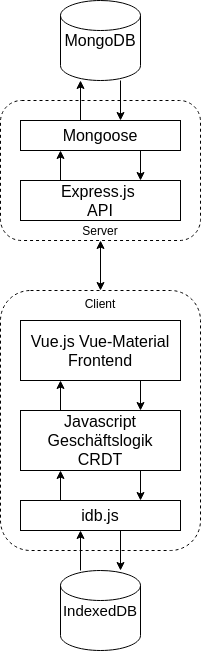
\includegraphics[width=0.33\textwidth]{architektur.png}
	\caption{Architektur des Prototypen}
	\label{fig:architektur}
\end{figure}

Abbildung \ref{fig:architektur} zeigt die Architektur des Prototypen. Die Clientseite setzt sich zusammen aus Frontend, Geschäftslogik und der Browser-API IndexedDB als lokalen Speicher. Zusätzlich wird die JavaScript-Bibliothek idb.js für den Zugriff auf IndexedDB genutzt. Die CRDT Funktionalitäten befinden sich in dieser Darstellung in der Geschäftslogik. 

Die Serverseite beginnt mit einer API, welche nur einen einzelnen Endpunkt (/sync) zur Synchronisierung von lokalen und Online-Daten bereitstellt. Über diese Schnittstelle kann der Client seine Operationen an den Server schicken und erhält als Antwort die gesammelten Operationen des Servers. Das server-seitige Speichern der Applikationen erfolgt auf einer MongoDB Datenbank. Ergänzend zu MongoDB wird noch die Bibliothek Mongoose genutzt. Als Laufzeitumgebung zum Betreiben des Webservers dient Node.js. Eine ausführliche Erläuterung, aus welchen Gründen die bestimmten Technologien genutzt werden, findet sich in Abschnitt \ref{sec:Technologien}.



\section{Entwurf der Nutzeroberfläche}

Aus den funktionalen Anforderungen (Abschnitt \ref{sec:funktionaleAnforderungen}) lässt sich ein Entwurf für die Nutzeroberfläche des Prototypen erstellen. Abbildung \ref{fig:rezepteFrame} zeigt den Hauptbildschirm der Website. Hier kann der Nutzer Rezepte hinzufügen, löschen und die Namen der angelegten Rezepte bearbeiten. Der \enquote{Sync} Button initialisiert das Synchronisieren mit dem Server. Über den Knopf \enquote{Zutaten} gelangt der Nutzer zur Übersicht der Zutaten des jeweiligen Rezepts. Wie auf Abbildung \ref{fig:zutatenFrame} zu erkennen ist, kann der Nutzer hier neue Zutaten für das Rezept anlegen und bestehende Zutaten bearbeiten oder löschen. Darüber hinaus kann er jeder angelegten Zutat eine Menge zuweisen und auch diese bearbeiten. 

\begin{figure}[H]
	\centering
	\begin{minipage}{.45\textwidth}
		\centering
		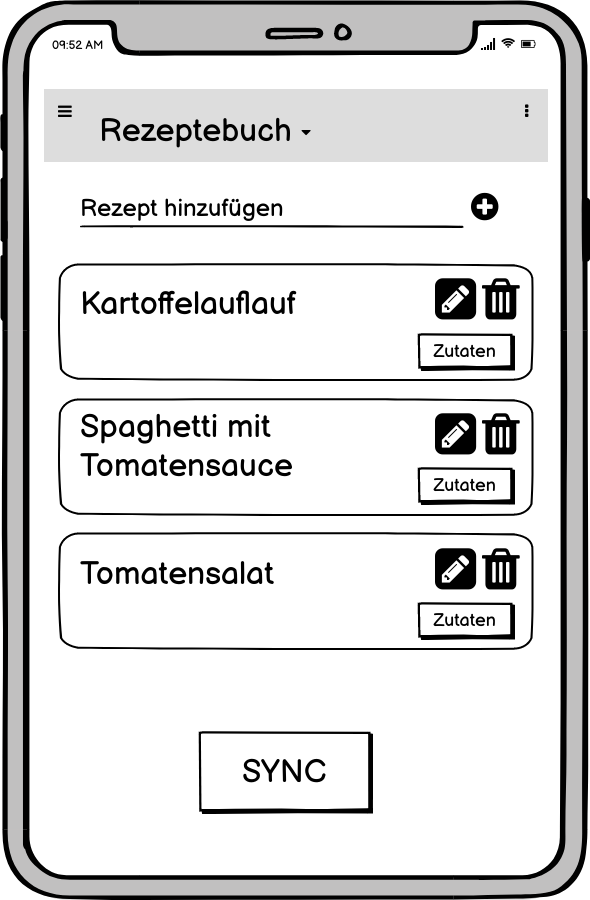
\includegraphics[width=1\textwidth]{wireframeRezepte2.png}
		\caption{Entwurf Nutzeroberfläche Hauptbildschirm}
		\label{fig:rezepteFrame}
	\end{minipage}
	\hspace*{\fill}
	\begin{minipage}{.45\textwidth}
		\centering
		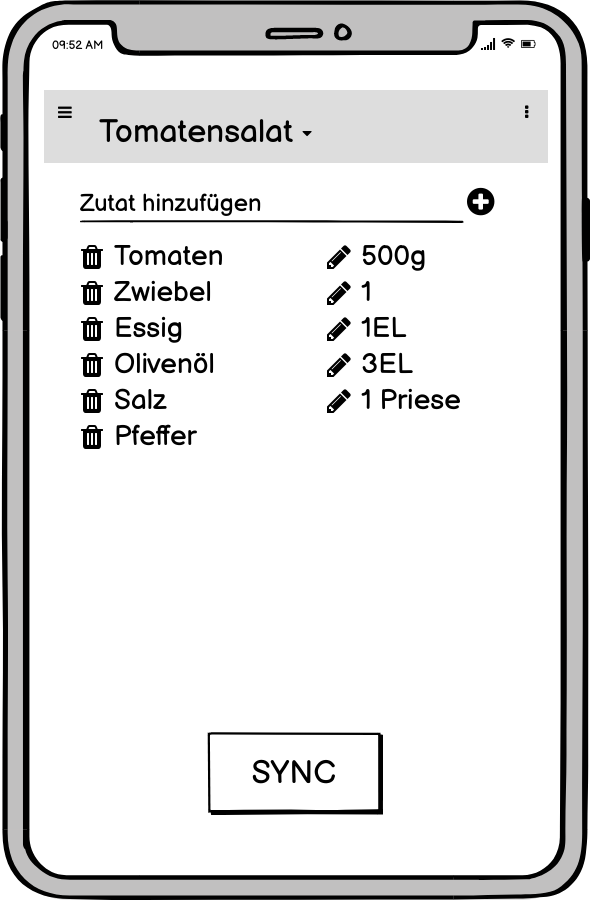
\includegraphics[width=1\textwidth]{wireframeZutaten2.png}
		\caption{Entwurf Nutzeroberfläche Zutaten}
		\label{fig:zutatenFrame}
	\end{minipage}
\end{figure}

\subsection{Optimistic UI}
\label{sec:optimisticUI}
Wenn der User eine Änderung über die Nutzeroberfläche einleitet, bekommt er diese schon zu sehen, bevor die Änderung in der Datenbank gespeichert wurde. Diese Praxis nennt sich Optimistic UI und ist ein gängiges Mittel um die Usability in modernen Applikationen zu steigern \autocite{ArticleOptimisticUI}.



\section{Datenstruktur}
\label{sec:Datenstruktur}

Dieser Abschnitt beschreibt die Planung der Datenstruktur für den Prototypen. Erster Schritt dieser Planung ist es, zu ermitteln, welche Daten von der Datenstruktur verwaltet werden müssen und wie diese von der Applikation genutzt werden. Das Vorgehen ist, die Grundlagen der Datenstruktur erst in konventionellen Datentypen zu entwerfen und diese anschließend um CRDT Funktionalitäten zu erweitern. Dies bietet sich an, da \acp{CRDT} üblicherweise auf konventionellen Datentypen aufbauen. Die Datenstruktur soll schließlich auf die Applikation zugeschnitten sein und nicht umgekehrt. Würde mit dem Entwurf des CRDT begonnen werden, bevor die Grundlagen der Applikation festgelegt sind, müsste sich die Applikation der Datenstruktur anpassen. Dies gilt es zu vermeiden, es sei denn, die Rahmenbedingungen fordern aus anderen Gründen eine bestimmte Datenstruktur, was in dieser Arbeit jedoch explizit nicht der Fall ist. Ziel des Prototypen ist es, die Datenstruktur an die Applikation anzupassen. 

\subsection{Grundlagen der Datenstruktur}

Die in Sektion \ref{sec:anforderungsanalyse} formulierten Anforderungen zeigen, dass es in der Applikation um das Speichern, Bearbeiten und Löschen von Rezepten und ihren Zutaten geht. Nun gilt es, zu modellieren, wie ein solches Rezept als Objekt in der Applikation aussieht. 

Listing \ref{lst:rezeptv1} zeigt die Struktur eines Rezeptes als einzelnes JavaScript Objekt. Neben einer ID verfügt es noch über die Eigenschaften \enquote{name}, welche den Namen des Rezepts speichert und die Eigenschaft \enquote{ingredients}. Bei \enquote{ingredients} handelt es sich um ein Array an Objekten, welche jeweils eine Zutat mit Namen (\enquote{name}) und Mengenangabe (\enquote{measure}) abbilden. Darüber hinaus erhält das Rezept zur Identifikation eine generierte ID. Da, wie in Sektion \ref{fig:architektur} erläutert, das lokale Speichern über die IndexedDB-API erfolgt, können die Rezepte auch direkt als Objekte in der Datenbank des Browsers gespeichert werden. Auch die Verschachtelung der Objekte stellt kein Problem dar, da IndexedDB auch Objekte mit Objekten als Eigenschaft speichert. Zwischen Applikation und lokalem Speichern muss folglich keine Umwandlung der Daten erfolgen.

%In diesem Modell ist ein Rezept schlussendlich ein verschachteltes Objekt und die gesamten Applikationsdaten lassen sich in einer Sammlung aller Rezepte finden. Übertragen auf abstrakte Datentypen wäre ein Rezept eine Map. Diese Map enthält die Schlüssel \enquote{name} und \enquote{ingredients}. Während zu dem Schlüssel \enquote{name} ein String als Wert gespeichert werden soll, dient der Schlüssel \enquote{ingredients} zur Speicherung der Zutaten des Rezeptes. Da ein Rezept mehr als eine Zutat haben kann, handelt es sich hierbei um ein Set. Dieses Set besteht wiederum aus den Zutaten Objekten, welche, genau wie das Rezept, Daten in Schlüssel-Wert Paaren beinhalten. Somit handelt es auch bei den Zutaten um Maps.

%Somit wäre ein Rezept schlussgefolgert eine Map, welche einen einzelnen Wert und ein Set speichert, welches wiederum eine unbestimmte Anzahl an Maps speichert, welche wiederum einzelne Werte speichern.

\begin{minipage}{\linewidth}
	\lstinputlisting[language=JavaScript, caption={Beispiel Rezept verschachtelt}, label={lst:rezeptv1}]{code/recipev1.js}
\end{minipage} 

Ein solches Modell ist nicht unüblich und gerade in JavaScript Anwendungen häufig praktisch, weil Objekte in diesen oft verschachtelt sind. Beim Einsatz von \acp{CRDT} jedoch lohnt es sich, die Datenstruktur so flach wie möglich zu gestalten. Wie in Abschnitt \ref{sec:CRDTs} beschrieben, bauen \acp{CRDT} auf herkömmlichen Datenstrukturen auf. Wenn es die Möglichkeit gibt, die Komplexität der ausgehenden Datenstruktur zu reduzieren, bedeutet dies auch eine Reduzierung an Komplexität für das zu implementierende CRDT.

Eine Option, die Datenstruktur abzuflachen, besteht darin, die in Listing \ref{lst:rezeptv1} gezeigten Daten zu normalisieren und somit relational abzubilden. In diesem Fall werden die Zutaten nicht als Array in dem Rezept verschachtelt, sondern werden einzeln gespeichert. Listing \ref{lst:rezeptv2} zeigt ein Rezept in der relationalen Modellierung, Listing \ref{lst:ingredientv2} eine dazugehörige Zutat. Die Verbindung zwischen Rezepten und Zutaten wird nun über die Eingenschaft \enquote{recipe} der Zutaten definiert. Hier wird die ID des Rezepts hinterlegt, welchem die Zutat zugehörig ist.

%TODO NORMALISIERUNG DARSTELLEN

\begin{minipage}{\linewidth}
	\lstinputlisting[language=JavaScript, caption={Beispiel Rezept relational}, label={lst:rezeptv2}]{code/recipev2.js}
\end{minipage}

\begin{minipage}{\linewidth}
\lstinputlisting[language=JavaScript, caption={Beispiel Zutat relational}, label={lst:ingredientv2}]{code/ingredientsv2.js}
\end{minipage}

\subsection{Erweiterung zum CRDT}
\label{sec:erweiterungCRDT}
Während sich bei konventionellen Datentypen nicht viel dadurch ändert, ob eine Zutat über \enquote{recipe.ingredient}, wie es in Listing \ref{lst:rezeptv1} der Fall wäre, oder \enquote{ingredient}, vgl. Listing \ref{lst:rezeptv2} angesprochen wird, wäre die Umsetzung als CRDT in der verschachtelten Variante deutlich komplexer. Die Ursache dafür ist, dass die Änderungen an Zutaten schließlich auch von CRDT-Funktionalitäten profitieren sollten. Das Modell für ein Rezept müsste deshalb als CRDT entworfen werden, welches ein weiteres CRDT als Eigenschaft hält. Dies ist in der Umsetzung durchaus möglich, in diesem Fall aber leicht durch die relationale Herangehensweise zu vermeiden.

Da in der Applikation kein universell einsetzbares CRDT entworfen werden soll, sondern eines, welches den Anforderungen der Anwendung gerecht wird, gilt es nun zu ermitteln, welche Schnittstellen es der Applikation zur Verfügung stellen muss. Aus der Anforderungsanalyse, welche in in Sektion \ref{sec:anforderungsanalyse} durchgeführt wurde, lassen sich die Anforderungen an das CRDT ableiten. Tabelle \ref{tab:crdtAnforderungen} fasst diese als Schnittstellen zusammen, welche die Datenstruktur der Applikation bereitstellen muss. 

\begin{table}[]
	\caption{CRDT Schnittstellen}
	\label{tab:crdtAnforderungen}
	\resizebox{\textwidth}{!}{%
		\bgroup
		\def\arraystretch{1,5}%
		\begin{tabular}{|l|l|}
			\hline
			\rowcolor[HTML]{EFEFEF} 
			Funktionale Anforderung & Anforderung an die Datenstruktur \\ \hline
			Anlegen von Rezepten & \begin{tabular}[c]{@{}l@{}}Verwaltung einer Sammlung von beliebig vielen Rezepten\\ Hinzufügen eines Rezepts in die Rezeptesammlung\end{tabular} \\ \hline
			Anlegen von Zutaten & \begin{tabular}[c]{@{}l@{}}Verwaltung einer Sammlung von  beliebig vielen Zutaten\\ Hinzufügen einer Zutat in die Zutatensammlung\end{tabular} \\ \hline
			Bearbeiten und Löschen & \begin{tabular}[c]{@{}l@{}}Bearbeitung der Eigenschaften Rezeptname, Zutatenname, Zutatenmenge\\ Entfernen eines Rezeptes aus der Rezeptesammlung\\ Entfernen einer Zutat aus der Zutatensammlung\end{tabular} \\ \hline
		\end{tabular}%
		\egroup
	}
\end{table}

Die Umsetzung im Prototypen erfolgt durch ein \enquote{Operation-based} CRDT. Da beide möglichen Formen gleichwertig sind (vgl. Abschnitt \ref{sec:stateopbased}) wurde diese Entscheidung getroffen weil \enquote{Operation-based} \acp{CRDT} unter Umständen eine geringere Nutzlast für HTTP-Requests und Responses bei der Synchronisierung verursachen. Dies liegt daran, dass \enquote{Operation-based} \acp{CRDT} nicht darauf angewiesen sind, ihren gesamten Zustand auszutauschen (vgl. ebenfalls Abschnitt \ref{sec:stateopbased}).

Wie in Sektion \ref{sec:stateopbased} erläutert, werden alle Änderungen, welche an den Applikationsdaten erfolgen, einzeln als Operationen abgespeichert. Wie Rezepte und Zutaten werden auch die Operationen über die IndexedDB-API lokal im Browser gespeichert. Neben der Funktion zum Erzeugen von Operationen muss das CRDT auch eine Funktion zum Anwenden der Operationen implementieren. 

Listing \ref{lst:operationv1} zeigt eine Operation, welche beim Umbenennen des in Listing \ref{lst:rezeptv2} entworfenen Rezeptes erzeugt und gespeichert wird. Die Felder \enquote{store}, \enquote{object} und  \enquote{key} dienen der Identifikation des Wertes, der geändert werden soll, \enquote{value} beschreibt den neuen Wert. Die dargestellte Operation dokumentiert also, dass im Object-Store \enquote{recipes} der Wert des Schlüssels \enquote{name} vom Objekt \enquote{re\_ckdiw1bxw002411w66m7mol85s} zu \enquote{Tomaten-Paprika-Salat} geändert werden soll. Darüber hinaus erhält die Operation noch eine eigene ID und einen Zeitstempel. Der Zeitstempel dient dazu, eine konfliktfreie Synchronisation zu gewährleisten, mehr dazu im nächsten Abschnitt. 

\begin{minipage}{\linewidth}
	\lstinputlisting[language=JavaScript, caption={Beispiel Operation}, label={lst:operationv1}]{code/operationv1.js}
\end{minipage}

\subsection{Parallele Änderungen}
\label{sec:paralleleÄnderungen}

Zwei Replikationen können sich synchronisieren, indem sie ihre gespeicherten Operationen austauschen. Nachdem eine Replikation über diesen Weg eingehende Operationen erhalten hat, müssen die Operationen auf die Applikationsdaten angewendet werden, damit die Änderungen einen Effekt haben. Nachdem eine eingehende Operation angewandt wurde, wird sie zu den lokalen Operationen abgespeichert.

Beim Anwenden der Operationen kann es vorkommen, dass zwei Operationen Änderungen am gleichen Wert vorgenommen haben. Für solche Fälle, genannt parallele Änderungen, müssen Regeln implementiert werden, um zu entscheiden, welche der parallelen Änderungen den Vorzug bekommt. Nur so ist gewährleistet, dass zwei Replikationen nach dem Synchronisieren auf dem gleichen Stand sind. Wäre die Auswahl zufällig oder würde sich stets die lokale Änderung durchsetzen, könnten die Applikationsdaten voneinander abweichen. So wäre Konvergenz zwischen den Replikationen und somit \ac{SEC} nicht gewährleistet und der Einsatz von \acp{CRDT} überflüssig.

Im Prototypen werden parallele Änderungen mit \ac{LWW} Regeln behandelt, wodurch sich einzelne Rezepte und Zutaten als LWW-Map Bezeichnen lassen (vgl. Abschnitt \ref{sec:lwwMap}). Abbildung \ref{fig:flwochartOperationen} zeigt, wie entschieden wird, ob eine eingehende Operation angewendet wird. Zuerst wird überprüft, ob es für eine eingehende Operation, welche angewendet werden soll, bereits eine lokale Operation gibt, welche denselben Wert betrifft. Ist dies der Fall, werden die Zeitstempel der aktuellsten lokalen Operation und der eingehenden Operationen verglichen. Ist die lokale Operation neuer als die eingehende Operation, wird die eingehende Operation ignoriert. Ist hingegen die eingehende Operation neuer, wird sie angewendet und anschließend, wie vorgesehen, zu den lokalen Operationen hinzugefügt. Dies verhindert auch das mehrfache Anwenden derselben Operation, wodurch das Verarbeiten eingehender Operationen idempotent ist. Dies ist eine wichtige Eigenschaft für das CRDT (vgl. Abschnitt \ref{sec:kommuassoidem}). 

\begin{figure}[H]
	\centering
	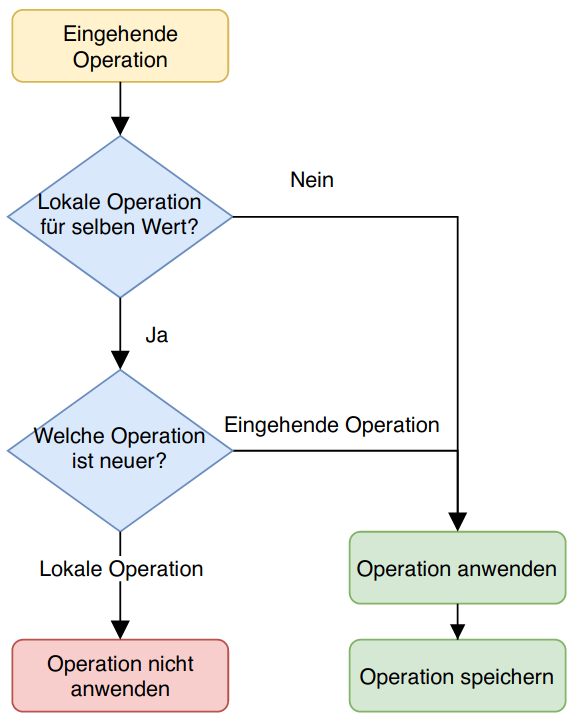
\includegraphics[width=0.6\textwidth]{flowchartOperationen.png}
	\caption{Bearbeiten einer eingehenden Operation}
	\label{fig:flwochartOperationen}
\end{figure}

\subsection{Anwenden von Operationen}
\label{sec:anwendenOperationen}

Auch beim Anwenden von Operationen gilt es, einigen potentiellen Fehlern aus dem Weg zu gehen. Da die Operationen kommutativ anwendbar sein sollen, kann es vorkommen, dass ein Objekt bearbeitet werden soll, welches lokal noch nicht existiert. Damit eine solche Änderung nicht verloren geht, wird das Objekt beim Anwenden der Änderung erstellt, sollte es noch nicht existieren. Wichtig hierbei ist, dass das neue Objekt keine zufällige ID zugewiesen bekommt, sondern die in der Operation hinterlegte ID des fehlenden Objektes. Anschließend kann die Operation wie vorgesehen auf das neue Objekt angewandt werden. Durch diese Semantik ist es möglich, die \enquote{Erstellen} und \enquote{Bearbeiten} Schnittstellen (vgl. Tabelle \ref{tab:crdtAnforderungen}) mit der gleichen Methode umzusetzen. Eine Operation zum Erstellen eines Objektes wird einfach genau wie eine Operation zum Bearbeiten angelegt, statt einer bestehenden ID beim Bearbeiten wird jedoch eine neue ID erzeugt. Somit wird das Objekt beim Anwenden der Operation erzeugt, da es sich um eine unbekannte ID handelt. 

Ein weiterer Fehlerfall droht beim Entfernen von Rezepten und Zutaten, welches neben dem Anlegen und Bearbeiten auch eine weitere Schnittstelle zur Datenstruktur ist (vgl. Tabelle \ref{tab:crdtAnforderungen}). Abbildung \ref{fig:rezeptLöschenSchlecht} zeigt die Problematik, welche auftritt, wenn das Objekt tatsächlich aus der Datenbank gelöscht wird. Wird ein Objekt gelöscht und anschließend bearbeitet, kommt die Applikation nicht auf den gleichen Stand wie, wenn die Operationen in umgekehrter Reihenfolge angewendet werden. Das liegt daran, dass das gelöschte Objekt beim anschließenden Bearbeiten wieder erzeugt wird. 

Somit wäre erneut das Kommutativgesetz verletzt und die Applikationsdaten könnten sich nach dem Synchronisieren unterscheiden. 

\begin{figure}[H]
	\centering
	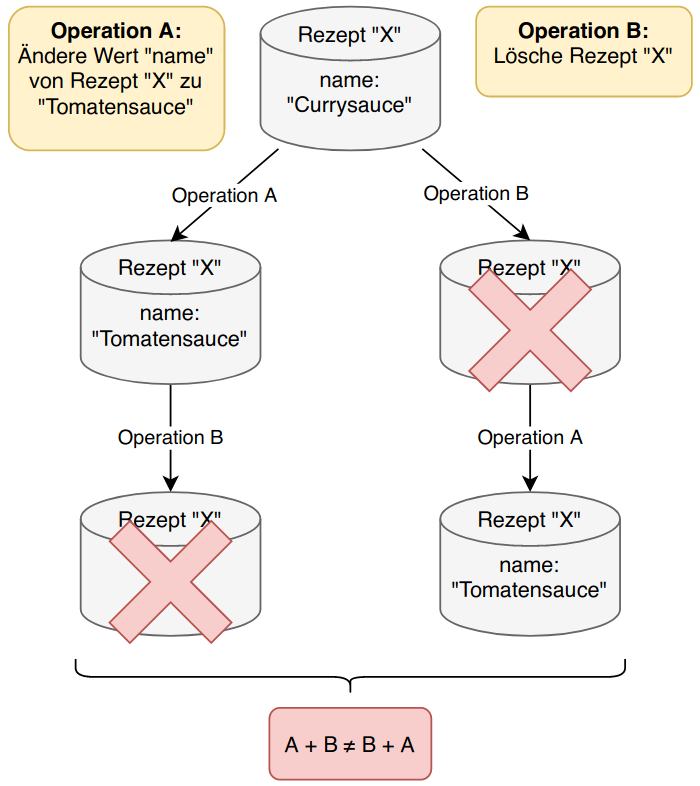
\includegraphics[width=0.66\textwidth]{deleteRecipeBad.png}
	\caption{Fehlerfall beim Entfernen eines Rezeptes}
	\label{fig:rezeptLöschenSchlecht}
\end{figure}

Im Prototyp werden die Rezepte- und Zutatensammlungen deshalb als G-Set (vgl. Sektion \ref{sec:g-set}) implementiert. Dies bedeutet, dass die Elemente des Sets, also die Rezepte und Zutaten, nicht mehr gelöscht werden können, nachdem sie einmal angelegt wurden. Stattdessen wird das Entfernen der Objekte über eine weitere Eigenschaft gelöst, den sogenannten \textit{tombstone}. Beim \textit{tombstone}, Englisch für Grabstein, handelt es sich um einen Statusindikator, welcher bestimmt, ob ein Objekt von der Applikation als aktiv oder inaktiv behandelt werden soll. Somit kann auch das Entfernen eines Objektes auf die gleiche Herangehensweise erfolgen wie das Anlegen und Bearbeiten.

\begin{minipage}{\linewidth}
	\lstinputlisting[language=JavaScript, caption={Beispiel Entfernen-Operation}, label={lst:operationv2}]{code/operationTombstone.js}
\end{minipage}

Listing \ref{lst:operationv2} zeigt, wie eine Entfernen-Operation ebenso Informationen über das Zielobjekt enthält. Der angesprochene Schlüssel ist dabei immer \textit{tombstone}, der Wert \enquote{1} indiziert, dass das Objekt als entfernt zu behandeln ist. Wäre eine Schnittstelle zum Reaktivieren des Objekts gewünscht, so könnte dies durch das Ändern des \textit{tombstone} Werts auf \enquote{0} umgesetzt werden. Abbildung \ref{fig:rezeptLöschenGut} zeigt, wie die Anwendung der vorher fehlerverursachenden Operationen durch die Nutzung des \textit{tombstone} Indikators wieder kommutativ ist.

\begin{figure}[H]
	\centering
	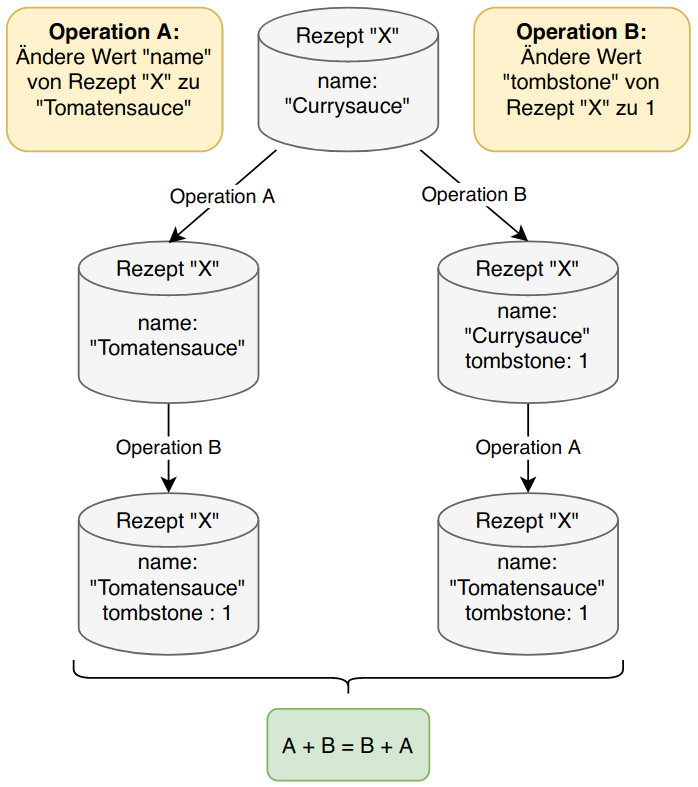
\includegraphics[width=0.66\textwidth]{deleteRecipeGood.png}
	\caption{Korrektes Entfernen eines Rezeptes}
	\label{fig:rezeptLöschenGut}
\end{figure}

\section{Server}

Da die Replikationen im Client-Server Modell nicht direkt miteinander kommunizieren können, ist es Aufgabe des Servers, dafür zu sorgen, dass dennoch Operationen ausgetauscht werden können. Dieser Abschnitt erläutert, wie der Server dazu genutzt wird, dass Clients indirekt miteinander kommunizieren können. 

\subsection{Aufgabe des Servers}
\label{sec:AufgabeServer}

Voraussetzung eines \enquote{operation-based} \acp{CRDT} ist es, die erzeugten Operationen verlässlich an die anderen Replikationen des Systems, im Falle des Prototypen also die anderen Clients, zu verteilen (vgl. Sektion \ref{sec:CRDTs}). Deshalb dient der Server in der Umsetzung des Prototypen als eine Art Cloud-Speicher für Operationen, auf dessen Schnittstelle alle Clients Zugriff haben. 

\subsection{API}

Die Schnittstelle, welche der Server den Clients bereitstellt, ist eine API mit genau einem Endpunkt. Bei diesem handelt es sich um eine POST-Route, welche ein Array an eingehenden Operationen als HTTP-Request akzeptiert. Nachdem die eingehenden Operationen vom Server verarbeitet wurden, werden die lokalen Operationen des Servers als HTTP-Response zurückgeschickt. 

\subsection{Datenbank}

Eingehende Operationen werden unter den gleichen Konditionen in der Datenbank des Servers gespeichert, wie sie in Abbildung \ref{fig:flwochartOperationen} beschrieben sind. Im Gegensatz zu dem Client wendet der Server jedoch keine Operationen an. Die Datenbank des Servers dient exklusiv der Speicherung von Operationen, Rezepte und Zutaten verwaltet er nicht. Dementsprechend muss die Datenbank des Servers keine weiteren Aufgaben erfüllen als das Lesen und Schreiben einer einzelnen Tabelle. 

\subsection{Synchronisation}

Um sich mit dem Server zu synchronisieren, schickt ein Client erst alle seine lokalen Operationen an den Server, um anschließend alle auf dem Server gespeicherten Operationen als Antwort zu bekommen.

\begin{figure}[H]
	\centering
	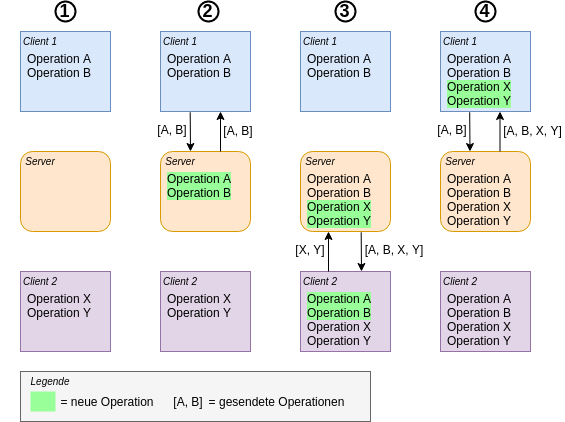
\includegraphics[width=1\textwidth]{syncDiagram2.png}
	\caption{Synchronisieren über den Server}
	\label{fig:syncDiagram}
\end{figure}

Abbildung \ref{fig:syncDiagram} demonstriert das Synchronisieren zweier Clients in vier Schritten. Diese lassen sich wie folgt beschreiben:

\begin{description}
	\item[Schritt 1] dokumentiert die Ausgangssituation. Beide Clients verfügen über unterschiedliche Operationen, während auf dem Server noch keine Operationen gespeichert sind. Für dieses Beispiel ist anzunehmen, dass Operationen A und B nicht die gleichen Werte bearbeiten wie Operationen X und Y, die Regeln für den Fall das gleiche Werte geändert werden, sind in Abschnitt \ref{sec:paralleleÄnderungen} erklärt.
	\item[Schritt 2] zeigt die Synchronisation von Client 1 und dem Server. Zuerst schickt der Client seine Operationen an den Server, welcher diese speichert, da die Operationen zuvor nicht in seiner Datenbank existierten. Als Antwort schickt der Server seine Operationen zurück. Dies hat jedoch keinen Effekt auf die Daten des Clients, da die gleichen Operationen zurückkommen, welche sich schon in der lokalen Datenbank befinden. Beim Bearbeiten eingehender Operationen (vgl. Abbildung \ref{fig:flwochartOperationen}) werden diese also ignoriert.
	\item[Schritt 3] beschreibt die anschließende Synchronisation von Client 2 und dem Server. Client 2 initiiert diesen, indem er seine Operationen X und Y an den Server sendet. Der Server speichert diese, da sie noch nicht in seiner Datenbank vorhanden sind und die Operationen andere Werte betreffen als Operationen A und B. Daraufhin antwortet der Server und schickt die Sammlung seiner gespeicherten Operationen zurück. Beim Bearbeiten der Operationen wendet Client 2 die neuen Operationen A und B an und speichert sie in seiner Datenbank. Die Operationen X und Y hingegen werden ignoriert, da diese schon in der Datenbank des Clients vorhanden sind.
	\item[Schritt 4] stellt dar, wie Client 1 sich erneut mit dem Server synchronisiert. Seit Schritt 1 hat sich auf dem Client nichts geändert, weshalb er die Synchronisation wieder mit dem Senden der Operationen A und B beginnt. Der Server kennt diese schon, fügt seiner Datenbank also keine Operationen hinzu und fährt fort, indem er seine Operationen an den Client sendet. In der Antwort des Servers sind nun auch die Operationen von Client 2 enthalten, welche den Server in Schritt 3 erreichten. Anschließend wendet Client 1 die eingehenden neuen Operationen X und Y an und speichert sie in seiner Datenbank. Somit sind Client 1 und Client 2 auf dem gleichen Stand. 
\end{description} 

\chapter{Prototypische Realisierung}

Dieses Kapitel beschreibt die Realisierung des Prototypen auf Basis des zuvor angefertigten Konzeptes. Zuerst wird auf die Wahl der bei der Umsetzung verwendeten Technologien eingegangen, anschließend folgen Erläuterungen zu den implementierten Funktionalitäten.

\section{Wahl der verwendeten Technologien}
\label{sec:Technologien}
Es folgt eine kompakte Vorstellung der zur Umsetzung des Prototypen genutzten Technologien. Auch wird erläutert, warum die einzelnen Technologien verwendet werden und welchen Einfluss sie auf die Implementierung des Prototypen haben.

\subsection{JavaScript, HTML und CSS}
JavaScript ist eine Skriptsprache welche zur clientseitigen Programmierung von Websites genutzt wird. Mit einer Nutzung in über 95\% \autocite{OnlineJavascriptDistr} aller Websites ist sie aus dem Internet nicht wegzudenken. In den letzten Jahren gewannen auch Sprachen an Popularität, die zu JavaScript kompilieren, wie zum Beispiel TypeScript oder ClojureScript. Da JavaScript die Basis dieser Sprachen bildet und sich gut in diese übersetzten lässt, ist eine Implementierung in der \enquote{Grundsprache} am besten dazu geeignet, die Anforderung einer anschaulichen und verständlichen Umsetzung zu erfüllen.
\subsection{VueJS}
\label{sec:vue}
Da es sich beim Prototypen nicht um eine statische Website handelt, sondern oft Änderungen an der Nutzeroberfläche oder an den Applikationsdaten vorgenommen werden, bietet sich die Nutzung eines Frameworks an, welches diese Interaktionen vereinfacht. 

VueJS ist ein JavaScript Framework zum Erstellen von Benutzeroberflächen. Die Nutzung von VueJS erlaubt die Verknüpfung von HTML-Elementen mit Anwendungsdaten. So können HTML-Elemente automatisch aktualisiert werden, wenn sich ein Wert in einem Vue-Objekt ändert. Diese Verknüpfung macht auch Änderungen in die umgekehrte Richtung möglich, also die Aktualisierung von Applikationsdaten bei Änderungen, welche auf Seite der Nutzeroberfläche gemacht werden.

Eine Funktionalität von VueJS ist die Erzeugung von \enquote{components}. Hierbei handelt es sich um VueJS Instanzen, welche in HTML wiederverwendet werden können. Bei der Umsetzung des Prototypen wird die Komponenten-Bibliothek vue-material genutzt, um Zugriff auf einige vorgefertigte Komponenten wie Cards, Buttons und Eingabefelder zu haben. 
\subsection{IndexedDB}
IndexedDB ist eine Browser-API, welche das clientseitige Speichern von Daten im Browser ermöglicht. Das bedeutet, dass über IndexedDB gespeicherte Daten der Applikation auch offline zur Verfügung stehen. Die Nutzung der IndexedDB Schnittstelle bietet dem Prototypen die Funktionalität der Speicherung von Offline-Daten, welche für die Erfüllung der funktionalen Anforderungen rund um Offline-First-Eigenschaften essenziell ist. 

Über sogenannte Object-Stores können JavaScript Objekte gespeichert und ausgelesen werden. Die Abfrage der Objekte erfolgt über einen der Werte des Objekts, welcher als Schlüssel konfiguriert wird. Alle Änderungen, welche an der Datenbank vorgenommen werden, erfolgen in Transaktionen. Änderungen an der Datenbank bestehen nur, wenn eine Transaktion erfolgreich war. Bei Komplikationen wird die Transaktion abgebrochen, wodurch die an der Datenbank während der Transaktion vorgenommenen Änderungen rückgängig gemacht werden. Somit bieten Transaktionen einen gewissen Schutz von Anwendungs- und Systemfehlern. Dies ist ein wichtiger Aspekt für die fehlerfreie Gewährleistung der CRDT-Funktionalitäten.
\subsection{idb}
\label{sec:idb}
Die Event- und Callback-basierte Schnittstelle, welche IndexedDB bietet, führt dazu, dass sehr komplexer Code geschrieben werden muss, um simple Operationen an der Datenbank durchzuführen \autocite{InproceedingsIDBdoof}. Um dieses Problem zu vermeiden und schlüssigen, lesbaren Code zu schreiben, wird bei der Umsetzung des Prototypen auf die JavaScript-Bibliothek idb zurückgegriffen. Bei idb handelt es sich um einen API-Wrapper, welche die API vereinfacht und Zugriff auf die Datenbank über JavaScript Promises anstelle von Events und Callbacks bietet. Listing \ref{lst:indexeddbexample} zeigt das Erzeugen eines Object-Stores über die gewöhnliche IndexedDB-API, in Listing \ref{lst:idbexample} ist die gleiche Aktion mit der idb API umgesetzt. Während in der gewöhnlichen Variante mit Callbacks weitergearbeitet werden muss, gibt die idb API mit \enquote{idb.open} ein Promise zurück.

\begin{minipage}{\linewidth}
	\lstinputlisting[language=JavaScript, caption=IndexedDB: öffnen eines Object-Stores, label={lst:indexeddbexample}]{code/indexedexample.js}
\end{minipage}

\begin{minipage}{\linewidth}
	\lstinputlisting[language=JavaScript, caption={idb: öffnen eines Object-Stores}, label={lst:idbexample}]{code/idbexample.js}
\end{minipage}

\subsection{Node.js, Express.js, MongoDB}
Obwohl die entwickelte CRDT Implementierung mit jeder Datenbank kompatibel ist, die Daten schreiben, lesen und suchen kann, wird zu demonstrativen Zwecken doch ein Node.js Server aufgesetzt, der mit einer MongoDB Datenbank verbunden ist. Node.js ist eine JavaScript Laufzeitumgebung, welche gewöhnlich zum Betreiben von Webservern genutzt wird. Für das Bereitstellen der einzelnen Route wird, wie üblich, Express.js genutzt. Die Datenbank muss, wie in Sektion \ref{sec:Architektur} erläutert, nur eine Tabelle für das Speichern von Operationen verwalten. Als Beispiel wird hier eine MongoDB Datenbank mit Mongoose als Object Data Modeling Bibliothek verwendet. Die Wahl fiel auf MongoDB, weil es eine populäre Datenbank ist. Funktionale Kriterien spielten bei der Wahl der Datenbank keine Rolle. 

\subsection{Sonstige Bibliotheken und Ressourcen}

\begin{description}
	\item[CUID] Die Bibliothek CUID wird zum Generieren der IDs von Rezepten, Zutaten und Operationen genutzt. Die IDs, welche als Primärschlüssel in den Datenbanken dienen, müssen einzigartig sein. Für diesen Zweck ist CUID in der Lage, kurze Strings zu erzeugen, welche mit Client-Fingerabduck, Timestamp, Counter und einer zufälligen Komponente aus mehreren kollisionsresistenten Elementen bestehen.
	\item[Roboto Font und Material Icons] Als Ergänzung zu den verwendeten vue-material Komponenten werden die Schrift Roboto und die SVG-Icons Material Icons von Google genutzt. Diese Assets sind komplett kosmetisch, sie passen schlicht gut zu den verwendeten Komponenten.
	\item[cors] Das node.js Paket cors wird genutzt, um \ac{CORS} zwischen Client und Server zu ermöglichen.
	%TODO hier fFußnote
\end{description}

\subsection{Ordnerstruktur}

Abbildung \ref{fig:ordnerstruktur} zeigt die Ordnerstruktur des Clients. Neben den für Webanwendungen üblichen Bestandteilen Template (index.html) und Stylesheet (app.css) ist die JavaScript Komponente des Prototypen in drei Dateien aufgeteilt. Sinn dieser Aufteilung ist es, die implementierten Funktionalitäten thematisch zu ordnen, einen praktischen Nutzen hat sie nicht. In app.js befinden sich Daten und Funktionalitäten, welche das Frontend betreffen. Die Datei crdt.js umfasst die Schnittstellen und Logik des implementierten \acp{CRDT}. In database.js befinden sich die Methoden, welche zum Zugriff auf die IndexedDB Datenbank umgesetzt wurden. 

Der implementierte Service-Worker befindet sich in sw.js. Darüber hinaus enthält der Client noch die Bibliothek idb.js. Die weiteren genutzten externen Ressourcen Vue.js, vue-material, CUID, Material Icons und die Roboto-Schrift werden über für prototypische Entwicklung übliche Content Delivery Networks in der index.html geladen.

\begin{figure}[H]
	\centering
	\begin{minipage}{.3\textwidth}
		\dirtree{%
			.1 crdt-app.
			.2 index.html.
			.2 app.js.
			.2 crdt.js.
			.2 database.js.
			.2 app.css.
			.2 sw.js.
			.2 ext.
			.3 idb.js.
		}
	\end{minipage}
	\caption{Ordnerstruktur des Clients}
	\label{fig:ordnerstruktur}
\end{figure}

	
\section{Nutzeroberfläche}

Die Nutzung von Vue.js ermöglicht die Erzeugung sogenannter Vue Instanzen. Diese Instanzen dienen dem Template als eine Art interaktives Viewmodel (vgl. Sektion \ref{sec:vue}). Im Prototypen wird eine Instanz zur Darstellung der gesamten Applikation mit dem Namen \enquote{app} erzeugt. Weitere Komponenten werden aus der Bibliothek vue-material genutzt.

Listing \ref{lst:htmlrecipes} zeigt, wie die Verwendung von Vue.js eine Verbindung von Anzeige und Applikationsdaten ermöglicht. Mit der Direktive \enquote{v-for} wird für jedes Rezept, welches sich in der visibleRecipes Eigenschaft der \enquote{app} Instanz befindet, ein <md-card> Block erzeugt. Bei <md-card> handelt es sich um eine vue-material Komponente. Innerhalb dieser Komponente kann nun auf die Eigenschaften des verbundenen Rezeptes zugegriffen werden. In diesem Fall wird beispielsweise der Name des jeweiligen Rezeptes als Titel der Komponente gesetzt.

Eine weitere Funktionalität, die Vue.js zur Verfügung stellt, ist \enquote{v-on:click}. Hierbei handelt es sich um einen Klick-Event-Listener, welcher direkt in ein HTML-Element geschrieben werden kann. Der Wert der Direktive definiert, welche Funktion ausgeführt wird, wenn auf das Element geklickt wurde. In Listing \ref{lst:htmlrecipes} ist zu sehen, wie so das Bearbeiten des Rezeptnamens (vgl. Zeile 7), das Löschen des Rezeptes (vgl. Zeile 11) und die Verlinkung zu den Zutaten des Rezeptes (vgl. Zeile 16) gesteuert werden. An jede der hier über \enquote{v-on:click} aufgerufenen Methoden wird das Rezept, mit welchem die Komponente verbunden ist, als Parameter übergeben. 

\begin{minipage}{\linewidth}
	\lstinputlisting[language = Html5, caption={HTML-Code der Rezepteliste}, label={lst:htmlrecipes}]{code/recipelist.html}
\end{minipage}

Neben der Auflistung an Rezepten verfügt die Hauptansicht der Applikation noch über ein Dialogfeld zum Anlegen der Rezepte und einen Button zum Synchronisieren der Applikationsdaten mit dem Server (vgl. Abbildung \ref{fig:uiMainSmall}). In der Zutatenübersicht eines Rezeptes (vgl. Abbildung \ref{fig:uiIngredientsSmall}) lassen sich Zutaten anlegen, Namen und Mengen bearbeiten und Zutaten löschen.

\begin{figure}[H]
	\begin{minipage}{.45\textwidth}
		\fbox{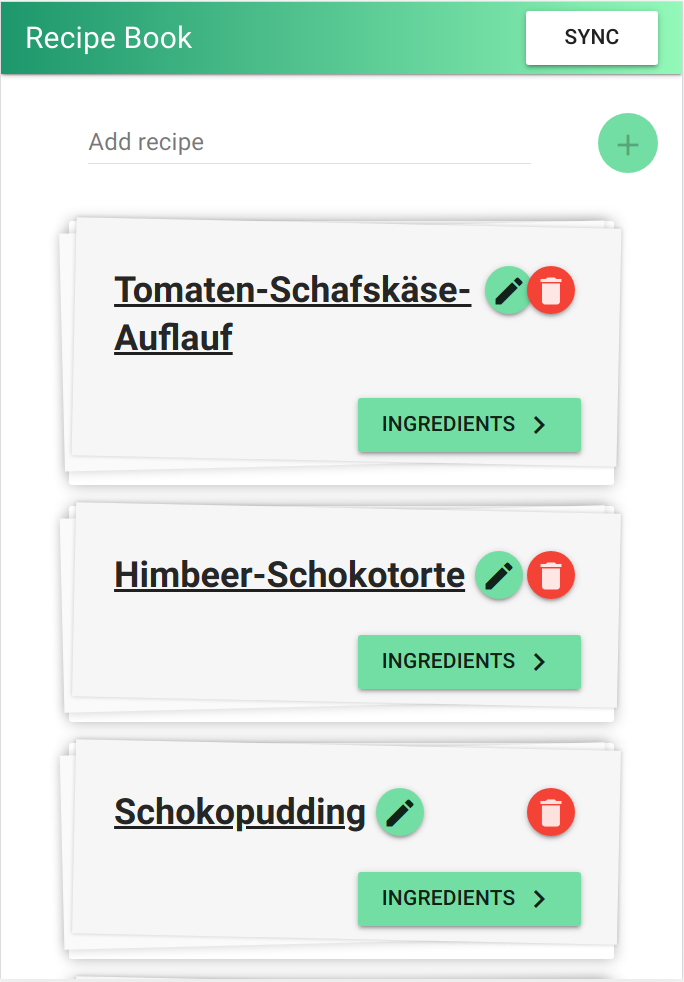
\includegraphics[width=1\textwidth]{uiMainSmall.png}}
		\caption{Hauptbildschirm}
		\label{fig:uiMainSmall}
	\end{minipage}
	\hfill
	\begin{minipage}{.45\textwidth}
		\fbox{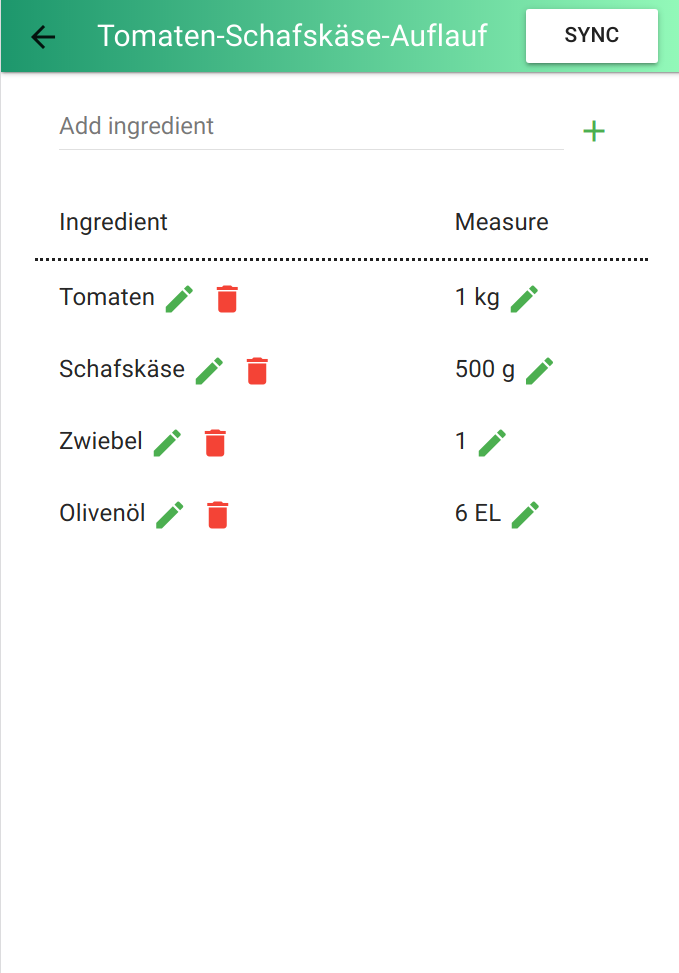
\includegraphics[width=1\textwidth]{ingredientsUISmall.png}}
		\caption{Übersicht Zutaten}
		\label{fig:uiIngredientsSmall}
	\end{minipage}
\end{figure}

\section{Service Worker}

Der Service Worker ermöglicht, dass der Prototyp nach dem ersten Laden der Applikation auch offline nutzbar ist. Hierzu werden alle Dateien, aus welchen der Client besteht, bei der Installation des Service Workers gecached (vgl. Listing \ref{lst:swinstall}). Die zu speichernden Ressourcen werden dabei als Parameter angegeben (vgl. Listing \ref{lst:swparameters}). Die Installation des Service Workers findet immer dann statt, wenn die Website geöffnet wird und noch kein Service Worker vorhanden ist.

\begin{minipage}{\linewidth}
	\lstinputlisting[language = Javascript, caption={Installation des Service Workers}, label={lst:swinstall}]{code/sw-install.js}
\end{minipage}

\begin{minipage}{\linewidth}
	\lstinputlisting[language = Javascript, caption={Parameter zur Installation des Service Workers}, label={lst:swparameters}]{code/sw-parameters.js}
\end{minipage}

Das Bereitstellen der Dateien aus dem Cache erfolgt über das Abfangen von Netzwerk-Requests. Das \textit{fetch} Event, für welches der in Listing \ref{lst:swintercept} dargestellte Event Listener registriert wird, feuert jedes Mal, wenn eine Ressource im Anwendungsbereich\footnote{Im Fall des Prototypen umfasst der Anwendungsbereich die gesamte Applikation} des Service Workers aus dem Netzwerk abgerufen werden soll. Dies bezieht sich sowohl auf Dokumente innerhalb des Anwendungsbereiches, wie die bei der Initialisierung gecacheten Dateien, als auch auf \textit{fetch} Requests an externe Ressourcen.

Wenn der Service Worker einen Request zum Synchronisieren abfängt, wird der Request nie vom Cache bedient, sondern immer an das Netzwerk weitergeleitet, wie im if-Block von Listing \ref{lst:swintercept} zu erkennen ist. Eine Synchronisierung muss schließlich stets mit neuen Daten erfolgen, ein erneutes Synchronisieren mit alten Daten hätte keine Auswirkung. Wenn keine Netzwerkverbindung besteht, funktioniert das Synchronisieren also auch nicht.

Um das Laden der Applikation so schnell wie möglich zu gestalten, ist der Service Worker für alle anderen Requests so konfiguriert, dass er eine \enquote{Cache dann Netzwerk} Strategie (vgl. Sektion \ref{sec:cachedannnetzwerk}) verfolgt. Im else-Block wird überprüft, ob sich die zum Request passende Response bereits im Cache befindet. Nur wenn dies nicht der Fall ist, wird der Request über das Netzwerk bearbeitet.

\begin{minipage}{\linewidth}
	\lstinputlisting[language = Javascript, caption={Service Worker: Abfangen von Requests}, label={lst:swintercept}]{code/sw-interceptRequests.js}
\end{minipage}

Im Prototypen ist dieses Verhalten wie folgt umgesetzt: 
Beim Aufrufen der Webseite werden alle lokal gespeicherten Applikationen aus der Datenbank geladen (vgl. Listing \ref{lst:loaduidata1}) und in zwei lokalen Variablen, \textit{recipes} und \textit{ingredients}, der \textit{app} Instanz gespeichert (vgl. Listing \ref{lst:loaduidata2}).

\begin{minipage}{\linewidth}
	\lstinputlisting[language = Javascript, caption={loadUIData Methode}, label={lst:loaduidata1}]{code/updateUI.js}
\end{minipage}

\begin{minipage}{\linewidth}
	\lstinputlisting[language = Javascript, caption={Laden aller Rezepte und Zutaten}, label={lst:loaduidata2}]{code/updateAllUI.js}
\end{minipage}

\section{Lokales Speichern über die IndexedDB-API}
\label{sec:lokalesIndexeddb}

Über die IndexedDB Schnittstelle müssen drei verschiedene Sätze an Daten lokal gespeichert werden: Rezepte, Zutaten und Operationen (vgl. Sektion \ref{sec:Datenstruktur}). Die Datensätze werden jeweils in einem eigenen ObjectStore in der Datenbank gespeichert. Listing \ref{lst:idbOpen} zeigt die Variable \enquote{idbPromise}, welche bei allen Zugriffen auf die Datenbank genutzt wird. Wie in Sektion \ref{sec:idb} erklärt, wird statt der üblichen IndexedDB-API die Promise-basierte Schnittstelle der idb.js Bibliothek genutzt. Beim jedem Zugriff auf die Datenbank wird geprüft, ob die ObjectStores bereits erstellt sind. Wenn dies nicht der Fall ist, werden sie angelegt. Nach erfolgreichem Öffnen der Datenbank gibt das Promise ein Objekt zurück, mit welchem Transaktionen an der Datenbank ausgeführt werden können.

\begin{minipage}{\linewidth}
	\lstinputlisting[language = Javascript, caption={Öffnen der IndexedDB Datenbank}, label={lst:idbOpen}]{code/idbOpen.js}
\end{minipage}

Somit können anschließend Zugriffe wie das Speichern von Objekten (vgl. Listing \ref{lst:saveObject}) oder das Abrufen aller Objekte eines ObjectStores (vgl. Listing \ref{lst:getAllFromStore}) erfolgen. Der Ablauf folgt dabei stets dem gleichen Muster. Zu Beginn wird die Datenbank mit dem \enquote{idbPromise} geöffnet, woraufhin eine Transaktion für den gewünschten ObjectStore erzeugt wird. Über die Transaktion ist schließlich der ObjectStore verfügbar, an welchem dann Daten ausgelesen oder geschrieben werden können.

\begin{minipage}{\linewidth}
	\lstinputlisting[language = Javascript, caption={Speichern eines Objektes im ObjectStore}, label={lst:saveObject}]{code/saveObject.js}
\end{minipage}

\begin{minipage}{\linewidth}
	\lstinputlisting[language = Javascript, caption={Abrufen aller Objekte eines ObjectStores}, label={lst:getAllFromStore}]{code/getAllFromStore.js}
\end{minipage}

\section{Generieren der Operationen}

Wie in Sektion \ref{sec:erweiterungCRDT} beschrieben, muss das CRDT über Methoden zum Generieren und Anwenden von Operationen verfügen. Welche Operationen generiert werden dürfen, ergibt sich aus den Anforderungen der Applikation. In der Konzeption (vgl. Tabelle \ref{tab:crdtAnforderungen}) wurden diese Anforderungen für den Prototypen definiert. Sie umfassen das Anlegen, Löschen und Bearbeiten von Rezepten und Zutaten. Da sich die Operationen zum Anlegen und Bearbeiten nicht unterscheiden müssen (vgl. Sektion \ref{sec:anwendenOperationen}) und das Löschen eines Objekts über das Bearbeiten des \textit{tombstone} Werts erfolgt, können alle drei Anforderungen über eine Methode erfüllt werden, die in Listing \ref{lst:generateUpdateOperation} aufgeführt ist. 

\begin{minipage}{\linewidth}
	\lstinputlisting[language = Javascript, caption={Funktion zum Generieren einer Operation}, label={lst:generateUpdateOperation}]{code/generateUpdateOperation.js}
\end{minipage}

Folgende Parameter müssen zum Generieren einer Operation übergeben werden: 
\begin{description}[leftmargin=!,labelwidth=\widthof{\bfseries store: }]
	\item [\textit{store:} ] Der ObjectStore, in dem sich das zu bearbeitende Objekt befindet. Im implementierten Prototypen gibt es die ObjectStores \enquote{recipes} und \enquote{ingredients}.
	\item [\textit{Id:} ] Die ID des Objektes, auf welches die Operation angewendet werden soll. Beim Anlegen eines Objektes muss zuvor eine neue CUID generiert werden.
	\item [\textit{key:} ] Der Schlüssel des Wertes, der bearbeitet werden soll, z.B. \enquote{name}.
	\item [\textit{value:} ] Der neue Wert.
\end{description}

Neben dem Mapping der übergebenen Parameter erzeugt die Methode noch einen aktuellen Zeitstempel und eine eigene CUID zum Identifizieren der Operation. Der Zeitstempel wird über die JavaScript Methode Date.now() erstellt, welche die Anzahl der vergangenen Millisekunden seit dem 01.01.1970 zurückgibt. Die Date.now() Methode orientiert sich an der Systemuhr des Clients, zu welcher es keine Garantie gibt, dass sie korrekt eingestellt ist. Im Rahmen der Entwicklung einer Anwendung, welche über einen Prototypen hinaus geht, sollten andere Methoden zur Erzeugung eines Zeitstempels genutzt werden, wie zum Beispiel die Implementierung einer Logischen Uhr, oder einer \ac{HLC}. Da das Vergleichen der Zeitstempel sich dabei jedoch nicht verändert, wurde aufgrund des begrenzten Umfangs und Zeitfensters bei der Implementierung des Prototypen auf die Umsetzung einer solchen Uhr verzichtet.

\section{Verarbeiten von Operationen}
\label{sec:processOperations}

Unabhängig davon, ob Operationen selbst erzeugt werden oder die Applikation über das Synchronisieren erreichen, werden sie konstant mit der gleichen Methode, \textit{processOperations}, verarbeitet. Es wäre zwar angemessen, davon auszugehen, dass eine gerade eben erstellte Operation immer neuer ist als andere lokale Operationen, und somit immer angewendet werden muss. Ein sofortiges Anwenden solcher Operationen würde jedoch ein Risiko darstellen, denn somit gäbe es zwei Methoden zum Anwenden von Operationen, welche laut CRDT Anforderung beide immer das gleiche Ergebnis liefern müssten. Wenn es nur eine universelle Funktion zum Anwenden von Operationen gibt, ist hingegen sichergestellt, dass die Operation auf allen Clients gleichermaßen angewendet wird. Dies ist eine wichtige Garantie, um \ac{SEC} zwischen den Replikationen herzustellen.

Operationen, die angewendet werden sollen, werden als \textit{eingehende Operationen} bezeichnet, die bestehenden gespeicherten Operationen als \textit{lokale Operationen}.

Aufgrund der Länge der \textit{processOperations} Methode wird diese in der folgenden Beschreibung in drei Schritte unterteilt. Der Vorgang beginnt mit dem Laden der lokalen Operationen. Mithilfe dieser Operationen wird anschließend gefiltert, welche der eingehenden Operationen anzuwenden sind. Schlussendlich werden die gefilterten Operationen angewendet.

\subsection{Lokale Operationen laden}

Der Erste Schritt der \textit{processOperations} Funktion ist das Laden der lokalen Operationen. Dies ist notwendig, weil die eingehenden Operationen im weiteren Verlauf der Methode mit den lokalen Operationen verglichen werden müssen. Wie Listing \ref{lst:processOperations1} zeigt, erfolgt das Laden der lokalen Operationen mit der im vorherigen Abschnitt (vgl. \ref{sec:lokalesIndexeddb}) beschriebenen Funktion \textit{getAllFromStore}.

\begin{minipage}{\linewidth}
	\lstinputlisting[language = Javascript, caption={processOperations, Teil 1}, label={lst:processOperations1}]{code/processOperations1.js}
\end{minipage}

Sobald die lokalen Operationen geladen sind, wird mit der Methode \textit{mapOperations} (vgl. Listing \ref{lst:mapOperations}) noch eine Vorkehrung für das Filtern im nächsten Schritt getroffen. \textit{mapOperations} gibt ein Promise zurück, welches beim auflösen ein \textit{Map} Objekt zurückgibt. Eine \textit{Map} wird verwendet, da sie das auch Objekte als Keys erlaubt, in diesem Fall eignet sich dies perfekt um zwei Operationen gegenüberzustellen. Ziel ist es hier, zu jeder eingehenden Operation eine lokale Operation zu finden, deren Zielwert übereinstimmt. Zielwert bedeutet hier die Kombination aus ObjectStore, Objekt und Schlüssel. 

Die Methode beginnt mit der Erzeugung eines leeren \textit{Map} Objektes und der Sortierung der lokalen Operationen. Die Sortierung erfolgt nach den Zeitstempeln, wobei die aktuellsten Operationen, also die mit dem höchsten Zeitstempel, am Anfang des Arrays platziert werden. 

Anschließend wird für jede der eingehenden Operationen eine passende lokale Operation gesucht. Eine Operation ist \enquote{passend}, wenn sie den exakt gleichen Zielwert wie die eingehende Operation bearbeitet. Durch das vorherige Sortieren der lokalen Operationen ist sichergestellt, dass die erste gefundene passende Operation stets die neueste ist. Nachdem die erste passende Operation gefunden wurde, ist also kein weiteres Suchen notwendig.

Daraufhin werden die eingehende Operation und die passende, lokale Operation zu der zuvor initialisierten \textit{Map} hinzugefügt. Die eingehende Operation wird als Schlüssel gesetzt, die lokale Operation als Wert. Wenn keine passende lokale Operation gefunden wird, ist der Wert \textit{undefined}. Nachdem jede eingehende Operation entweder ein lokales Gegenstück oder \textit{undefined} zugeordnet bekommen hat, wird die nun gefüllte Map zurückgegeben. 

\begin{minipage}{\linewidth}
	\lstinputlisting[language = Javascript, caption={mapOperations Methode}, label={lst:mapOperations}]{code/mapOperations.js}
\end{minipage}

\subsection{Operationen filtern}
\label{sec:filtern}

Mit der zurückgegebenen Map von eingehenden zu lokalen Operationen kann das Filtern beginnen. In \textit{processOperations} werden die \textit{mappedOperations} nun an die Funktion \textit{filterOperationsToApply} weitergegeben (vgl. Listing \ref{lst:processOperations2}).

\begin{minipage}{\linewidth}
	\lstinputlisting[language = Javascript, caption={processOperations, Teil 2}, label={lst:processOperations2}]{code/processOperations2.js}
\end{minipage}

Ziel des Filterns ist es, zu ermitteln, ob die eingehenden Operationen angewendet werden dürfen oder nicht. Die Regeln, nach welchen entschieden wird, welche Operationen angewendet werden und welche nicht, werden aus der Konzeption übernommen (vgl. Abbildung \ref{fig:flwochartOperationen}). Das vorherige Zuordnen der lokalen zu den eingehenden Operationen erleichtert diesen Vorgang, da somit nicht während des Filterns nach den passenden lokalen Operationen gesucht werden muss. Technisch wäre es zwar durchaus möglich, das Zuordnen von lokalen zu eingehenden Operationen während des Filterns durchzuführen, die Konsequenz wäre jedoch verschachtelter, schwer lesbarer Code.

Listing \ref{lst:filterOperations1} zeigt den Code für das Filtern der Operationen, auf Abbildung \ref{fig:filterOperationsFlowchart} ist der Vorgang noch einmal bildlich dargestellt. Das Filtern beginnt mit dem Initialisieren zweier Arrays, eines zum Halten der Operationen für Rezepte, ein weiteres für Operationen, die sich auf Zutaten beziehen. Anschließend läuft eine for-Schleife über jeden Schlüssel, also jede eingehende Operation, der \textit{mappedOperations} Map. In jeder Iteration der for-Schleife wird über die Zeitstempel geprüft, ob die eingehende Operation aktueller ist als die passende lokale Operation. Ist dies der Fall, wird die eingehende Operation zu dem jeweils passenden Array hinzugefügt. Dies passiert ebenso, wenn keine passende lokale Operation vorhanden ist und der Wert stattdessen \textit{undefined} ist. Wenn ein Wert in der Map \textit{undefined} ist, bedeutet es schließlich, dass das Objekt noch nicht existiert und angelegt werden muss. Diese Operationen müssen also immer angewendet werden. 

\begin{minipage}{\linewidth}
	\lstinputlisting[language = Javascript, caption={Filtern der Operationen, Teil 1}, label={lst:filterOperations1}]{code/filterOperations1.js}
\end{minipage}

\begin{figure}[H]
	\centering
	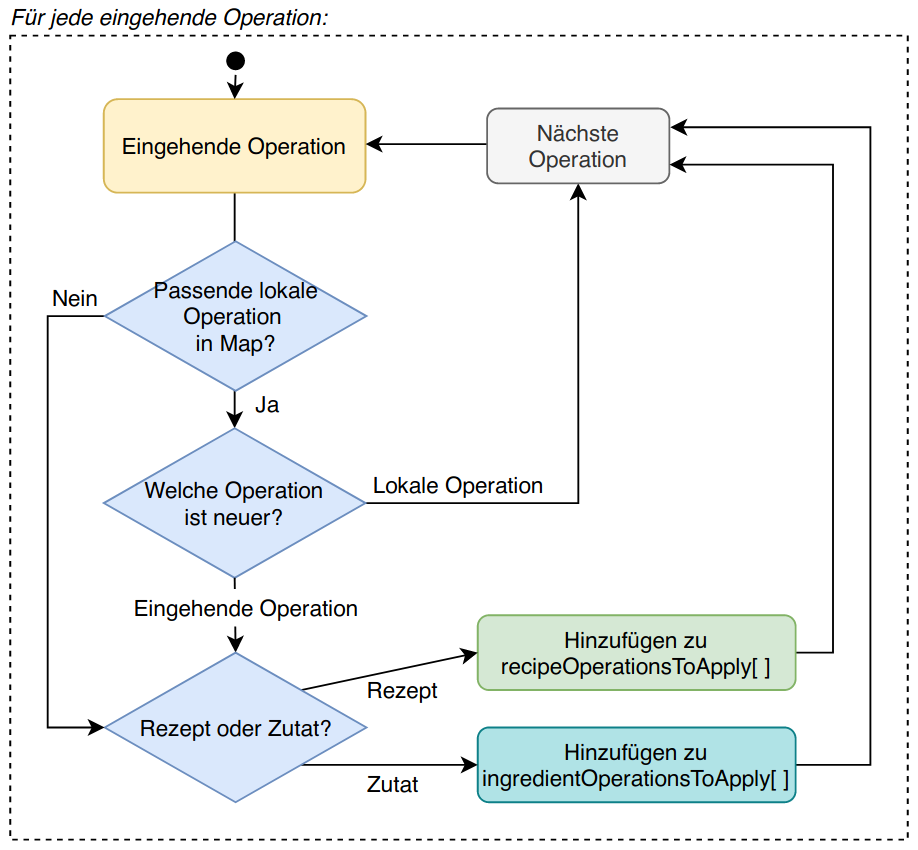
\includegraphics[width=.80\textwidth]{flowchartFilterOperations.png}
	\caption{Filtern der Operationen}
	\label{fig:filterOperationsFlowchart}
\end{figure}

Nachdem alle eingehenden Operationen die for-Schleife durchlaufen haben, werden die beiden Arrays \textit{recipeOperationsToApply} und \textit{ingredientOperationsToApply} in der Map \textit{operationsToApply} gespeichert (vgl. Listing \ref{lst:filterOperations2}). Schlüssel der in der Map gespeicherten Arrays ist jeweils der Name des ObjectStores. Dies geschieht, damit alle Operationen sich weiterhin in einem Objekt befinden und somit das Promise, welches \textit{filterOperationsToApply} zurückgibt, einen einzelnen Rückgabewert hat. Anschließend kann so die Promise-chain\footnote{Aneinanderreihung mehrerer Promises über das wiederholte Aufrufen der \textit{.then} Methode des jeweils vorherigen Promises} zum Verarbeiten der Operationen nahtlos fortgeführt werden, ohne Kompromisse zum Nutzen mehrerer Rückgabewerte treffen zu müssen.

\begin{minipage}{\linewidth}
	\lstinputlisting[language = Javascript, caption={Filtern der Operationen, Teil 2}, label={lst:filterOperations2}]{code/filterOperations2.js}
\end{minipage}

\subsection{Operationen anwenden}

Sobald das Filtern der Operationen abgeschlossen ist, kann mit dem Anwenden der Operationen begonnen werden. Die Map, welche von \textit{filterOperationsToApply} zurückgegeben wurde, enthält nun Operationen, die definitiv angewendet werden müssen, zugeordnet zum jeweiligen ObjectStore. Diese Operationen werden im Folgenden als \textit{valide Operationen} bezeichnet. Als Beispiel, wie diese Struktur in der Anwendung aussieht, zeigt Abbildung \ref{fig:validOperationsMapChrome} eine \textit{validOperationsMap} mit vier validen Operationen für Rezepte und sechs validen Operationen für Zutaten.

\begin{figure}[H]
	\centering
	\fbox{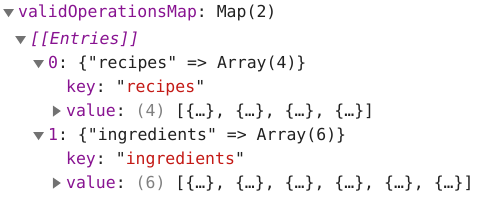
\includegraphics[width=.6\textwidth]{validOperationsMapChrome.png}}
	\caption{\textit{validOperationsMap} im Chrome-Debugger}
	\label{fig:validOperationsMapChrome}
\end{figure}

Listing \ref{lst:processOperations3} zeigt die Fortsetzung der \textit{processOperations} Methode durch Verschachtelung zweier \textit{Promise.all}\footnote{Die \textit{Promise.all} Methode nimmt mehrere Promises als Input und gibt ein einzelnes Promise zurück, welches zu einem Array der Ergebnisse aller Input-Promises auflöst. Das zurückgegebene Promise wird nur aufgelöst, nachdem alle Input-Promises erfolgreich aufgelöst wurden. Wird eines der Input-Promises abgelehnt, ist auch sofort das Rückgabe-Promise abgelehnt.} Methoden. Was auf den ersten Blick komplex aussieht, ist in der Praxis relativ einfach.

\begin{minipage}{\linewidth}
	\lstinputlisting[language = Javascript, caption={Verarbeiten der Operationen, Teil 3}, label={lst:processOperations3}]{code/processOperations3.js}
\end{minipage}

Die erste \textit{Promise.all} Methode bekommt für jeden Schlüssel in der \textit{validOperationsMap} eine weitere \textit{Promise.all} Methode als Input. Diese weiteren \textit{Promise.all} Methoden bekommen für jede Operation in dem entsprechenden ObjectStore ein \textit{updateObject} Promise als Input. Das erste \textit{Promise.all} sorgt also dafür, dass jeder ObjectStore, der aktualisiert werden muss, aktualisiert wird. Die weiteren \textit{Promise.all} Methoden, jeweils eine pro ObjectStore, stellen sicher, dass für jede Operation die \textit{updateObejct} Methode aufgerufen wird.

\begin{minipage}{\linewidth}
	\lstinputlisting[language = Javascript, caption={updateObject Methode, Teil 1}, label={lst:updateObject}]{code/updateObject.js}
\end{minipage}

In \textit{updateObject} (vgl. \ref{lst:updateObject}) wird das Objekt, auf das die Operation angewendet wird, zuerst aus der Datenbank geladen. Dies ist nötig, weil es nicht möglich ist, einzelne Werte eines Objektes über die IndexedDB-Schnittstelle zu ändern, ohne die anderen Werte des Objektes dabei zu verlieren. Deshalb ist es üblich, erst das komplette Objekt zu laden, dieses anschließend zu modifizieren, um schlussendlich die modifizierte Version in der Datenbank zu speichern und die alte Version zu überschreiben. So geschieht es auch in der \textit{updateObject} Methode, welche nach dem Laden des Objektes die Funktion \textit{modifyObject} (vgl. Listing \ref{lst:modifyObject}) aufruft. 

\begin{minipage}{\linewidth}
	\lstinputlisting[language = Javascript, caption={modifyObject Methode}, label={lst:modifyObject}]{code/modifyObject.js}
\end{minipage}

Es kann vorkommen, dass das Objekt, welches modifiziert werden soll, noch nicht existiert (vgl. Abschnitt \ref{sec:erweiterungCRDT}). Ist dies der Fall, gibt das Laden des Objektes im vorherigen Schritt \textit{undefined} zurück. In dieser Situation muss das Objekt in der \textit{modifyObject} Methode erst erstellt werden, bevor die Operation angewendet werden kann. Diese Anforderung ist auch in der Konzeption festgehalten (vgl. Abbildung \ref{fig:flwochartOperationen}).

Anschließend wird die Operation angewendet, indem der Wert des in der Operation definierten Schlüssels mit dem neuen Wert überschrieben wird. Die Operation wird nun über die \textit{saveObject} Funktion (vgl. Sektion \ref{sec:lokalesIndexeddb}) in der Datenbank der lokalen Operationen gespeichert.

Zurück in der \textit{updateObject} Methode steht nur noch das Speichern des modifizierten Objektes an. Dies erfolgt über die gleiche Methode, mit welcher zuvor schon die Operation gespeichert wurde.

\section{Synchronisieren}

Zum Synchronisieren werden Operationen zwischen Client und Server über eine API (siehe Sektion \ref{sec:Architektur}) ausgetauscht. In diesem Abschnitt wird beschrieben, wie diese Funktionalität auf Client und Server implementiert ist.

Das Synchronisieren beginnt auf Seite des Clients mit dem Abrufen aller lokalen Operationen (vgl. Listing \ref{lst:sync}). Sind die Operationen erfolgreich abgerufen, werden sie über den \textit{/sync} Endpunkt der API an den Server geschickt. 

\begin{minipage}{\linewidth}
	\lstinputlisting[language = Javascript, caption={Synchronisation Client}, label={lst:sync}]{code/sync.js}
\end{minipage}

Auf dem Server werden die Operationen nach den gleichen Kriterien verarbeitet wie die Operationen des Clients (vgl. Abbildung \ref{fig:flwochartOperationen}) mit dem Unterschied, dass der Server die Operationen nur speichern und nicht anwenden muss (vgl. Abschnitt \ref{sec:AufgabeServer}). Über die MongoDB Funktion \textit{insertMany} können alle Operationen auf einmal in die Datenbank geschrieben werden (vgl. Listing  \ref{lst:server1}). Wenn eine Operation bereits in der Datenbank existiert, wird sie mit \textit{insertMany} nicht erneut gespeichert. Zwar meldet MongoDB bei solchen Fällen einen Fehler, doch mit der Option \textit{ordered: false} können diese ignoriert werden.

Nach dem Speichern der eingehenden Operationen werden die lokalen Operationen des Servers mit der MongoDB Funktion \textit{find} geladen und anschließend als HTTP-Response an den Client geschickt. Auf diesem werden die eingehenden Operationen nun mit der \textit{processOperations} Methode (siehe Abschnitt \ref{sec:processOperations}) verarbeitet.

\begin{minipage}{\linewidth}
	\lstinputlisting[language = Javascript, caption={Synchronisation Server}, label={lst:server1}]{code/server1.js}
\end{minipage}

\section{Löschen überflüssiger Operationen}

Durch das ständige Hinzufügen von Operationen droht die Kommunikation zwischen Client und Server auf Dauer immer langsamer zu werden. Um dies zu verhindern, sind sowohl im Client als auch im Server Maßnahmen zur Reduzierung der Menge an Operationen implementiert.

Kommt es beim Verarbeiten der Operationen vor, dass zwei Operationen dieselbe Kombination aus ObjectStore, Objekt, Schlüssel und Wert haben, setzt sich immer die aktuellere der beiden Operationen durch. In der Implementierung des Prototypen wird sich die ältere Operation nie gegen die aktuelle durchsetzen, was bedeutet, dass die ältere Operation irrelevant ist. Deshalb wird die alte Operation diesem Fall gelöscht. 

Auf dem Client findet das Löschen alter Operationen während des Filterns der Operationen statt (vgl. Abschnitt \ref{sec:filtern}). In diesem Schritt werden die lokalen Operationen schließlich ohnehin mit den eingehenden Operationen verglichen.

\begin{minipage}{\linewidth}
	\lstinputlisting[language = Javascript, caption={Löschen überflüssiger Operationen auf dem Client}, label={lst:deleteUselessOpCluient}]{code/deleteUselessOpClient.js}
\end{minipage}

\chapter{Evaluation}

In diesem Abschnitt wird die Umsetzung der funktionalen und nicht-funktionalen Anforderungen reflektiert und auf Funktionsfähigkeit und Vollständigkeit überprüft.

\section{Anlegen, Bearbeiten und Löschen von Rezepten und Zutaten}
Das Anlegen, Bearbeiten und Löschen von Rezepten und Zutaten funktioniert über das implementierte CRDT. Somit können diese Aktionen von der Applikation vorgenommen werden, ohne dabei direkt die Anwendungsdaten zu verändern. Stattdessen nutzt die Applikation die Schnittstelle des \acp{CRDT} zum Generieren von Operationen, welche anschließend mit der \textit{processOperations} Methode angewendet werden können.

Die Anforderungen zum Bearbeiten und Anlegen der Objekte sind im Prototypen vollständig erfüllt, sollte dieser jedoch um komplexere Datenstrukturen erweitert werden, müsste auch das CRDT nachziehen. Da ein \ac{G-Set} umgesetzt wurde, findet das Löschen eines Objekts nicht wirklich statt, stattdessen wird die Sichtbarkeit des Objektes über einen Indikator gesteuert. Somit wächst die Menge der gespeicherten Daten konstant. Auf die Funktionalität des Prototypen hat dies zwar keine Auswirkung, da die gespeicherten Datenmengen winzig sind. Für große, skalierbare Projekte sollte jedoch auf eine andere Methodik zum Löschen gesetzt werden.

\section{Zugriff mit mehreren Endgeräten zugleich}
Mehrere Nutzer können zur gleichen Zeit auf die selbe Applikation zugreifen. Solange sie nicht den exakt gleichen Wert bearbeiten, sorgt die CRDT-basierte Synchronisierung dafür, dass niemand seine Arbeit verliert. Der gewählte Weg der \ac{LWW} Konfliktlösung ist ein Kompromiss, der für die Anwendung am meisten Sinn ergibt. Es sollte immer individuell entschieden werden, welche Art der Lösung für gleichzeitige Änderungen desselben Wertes am besten zu den Anforderungen der Applikation passt.
%TODO EVTL SCHLUSS FAZIT

\section{Offline Erreichbarkeit}
Die Offline Erreichbarkeit wird durch die Implementierung eines Service-Workers ermöglicht. Die Applikation ist offline vollständig funktionsfähig, nur das Synchronisieren über den Server funktioniert natürlich nicht, wenn der Server nicht erreichbar ist. Der Service Worker konnte gezielt so konfiguriert werden, dass die HTTP-Requests an den Server ignoriert werden.

\section{Lokales Speichern}
Für das lokale Speichern wird IndexedDB genutzt. Da der direkte Weg über die IndexedDB-API unnötig komplex erscheint, nutzt der Prototyp die Bibliothek idb.js. Diese ermöglicht durch das Bereitstellen von Promises, einen sehr angenehmen Umgang mit der Schnittstelle. Somit können die Anwendungsdaten offline und online problemlos gespeichert und ausgelesen werden.

\section{Synchronisierung von Daten und SEC}

Die Synchronisierung wird durch den Austausch von Operationen und das anschließende Anwenden eben dieser umgesetzt. Da die Clients nicht direkt miteinander kommunizieren, erfolgt dieses Austauschen über einen Server, welcher für alle Clients erreichbar ist. 

%TODO SCHLECHT
Während die Nutzung des API-Endpunktes zum Synchronisieren nur das Hin- und Herschicken von Operationen umfasst, sind die Methoden, welche die Synchronisierung ermöglichen, weitaus komplexer. Sie ermöglichen das Erzeugen und Verarbeiten der Operationen. Somit stellen die Schnittstelle zum CRDT dar, welches wiederum so konzipiert wurde, dass zwei Replikationen nach dem Synchronisieren tatsächlich konvergent sind.

Die Implementierung der Synchronisierung funktioniert für alle Änderungen an Daten, die der Nutzer vornehmen kann und ist somit in vollem Umfang erfüllt. Durch die eingebundenen Regeln bei der Anwendung von Operationen ist garantiert, dass sich zwei Clients, welche die gleichen Operationen angewendet haben, im gleichen Zustand befinden. Somit ist auch die Anforderung nach \ac{SEC} unter den Clients erfüllt. 

Ein interessanter Ansatz wäre, Synchronisation auch über andere Wege als den Server zu erlauben. Das Synchronisieren könnte schließlich auch von Client zu Client erfolgen, da hierfür lediglich das gegenseitige Austauschen der lokalen Operationen nötig ist.

\section{Konfliktfreies Synchronisieren}
Die Anforderung des konfliktfreien Synchronisierens ist nur teilweise erfüllt. Zwar werden zwei synchronisierte Clients immer den gleichen Zustand haben, dieser kann jedoch für beide Akteure fehlerhaft sein. Dies liegt an der Nutzung der \textit{Date.now} Methode. Da sie die Systemzeit des jeweiligen Endgerätes zum Erstellen von Zeitstempeln nutzt, ist nicht garantiert, dass die neueste Operation sich durchsetzt. Somit ist die umgesetzte \enquote{LWW} Regel fehleranfällig, wenn auf den Endgeräten der Clients inkorrekte Systemzeiten eingestellt sind.

Diese Anfälligkeit sollte sich jedoch mit der Nutzung einer \ac{HLC} beheben lassen. \ac{HLC} orientiert sich neben der Zeit auch an der Reihenfolge der Änderungen in der Applikation und kann somit als verlässlicher Zeitstempel in verteilten Systemen dienen \autocite[S. 1]{InproceedingsHLC}. 

%TODO QUELLE

\section{Unabhängigkeit von Datenbank-Technologien}

Im Entwickelten Prototypen muss keine der beiden Datenbanken, sowohl auf der Clientseite noch auf der Serverseite, Funktionalitäten für das Synchronisieren der Daten bereitstellen. Somit ist die Anforderung der Unabhängigkeit von Datenbank-Technologien erfüllt. 

Die Serverseitige Datenbank lediglich als zentraler Speicher von Operationen. Jede Datenbank, die in der Lage ist, Tabellen oder Objekte auszulesen und zu schreiben, sollte also qualifiziert sein, diese Aufgabe zu übernehmen. Auf der Clientseite gibt es für Webanwendungen derzeit keine Alternativen zur IndexedDB-API. 

%Entwickler lokaler Anwendungen, die nicht im Browser laufen, könnten jedoch auch eine beliebige lokale Datenbank nutzen.

\chapter{Fazit und Ausblick}

\section{Fazit}

Mit der Umsetzung des Prototypen wurde gezeigt, dass der Einsatz von CRDTs eine valide Lösung für die Synchronisierung von Applikationsdaten in Offline-First Anwendungen ist.

Bei der Planung der Datenstruktur ist es wichtig, die Anforderungen, welche die Applikation erfüllen muss, und somit auch die geplante Interaktion mit den Applikationsdaten zu kennen. Im Fall des Prototypen wird das CRDT aus einer Sammlung von Grow-Only Sets, welche wiederum LWW-Maps beinhalten, gebildet. Diese CRDTs sind in Komplexität und Funktionsumfang relativ simpel, eignen sich jedoch sehr gut für die flache Datenstruktur des Prototypen. Mit 204 Zeilen JavaScript Code, was zu einer Dateigröße von 6,9kb in ausgeschriebener Fassung und 2,1kb in minimierter Version führt, ist die Implementierung des CRDT Prototypen sehr Schlank. Herausforderungen zeigen sich bei der implementierten Datenstruktur noch in der Skalierbarkeit. In dieser Hinsicht bedenklich ist, dass die Elemente des G-Sets nicht gelöscht werden können und auch die Menge der Operationen, selbst mit regelmäßigem Löschen, kontinuierlich ansteigen dürfte. Auch bedarf der Prototyp einer Erweiterung um eine sichere Methode zum erzeugen von Timestamps, da die umgesetzte Nutzung von JavaScripts \textit{Date.now} nicht zuverlässig ist. Eine bekannte Lösung für dieses Problem wäre die Implementierung einer Hybrid-Logical-Clock (HLC).

Eine generelle Empfehlung zur Nutzung bestimmter CRDTs in Offline-First Webanwendungen lässt sich jedoch nicht aussprechen. Dies ist aber eher eine positive Erkenntnis, als eine negative. Wenn im Prototypen beispielsweise beim Synchronisieren das Bearbeiten stets das Löschen von Rezepten und Zutate überschreiben sollte, hat man als Entwickler die Möglichkeit das Verhalten des CRDTs anzupassen. Statt LWW-Maps würde sich dann die Umsetzung von Update-Wins-Maps anbieten. Die große Anzahl bereits erforschten, entwickelten und umgesetzten CRDTs bietet Webentwicklern eine gute Grundlage, sich passende Bausteine für die eigene, maßgeschneiderte Datenstruktur zu sichern. Dabei sollte beachtet werden, dass die Umsetzung von CRDTs nicht für jeden Anwendungsfall geeignet ist. Für komplexe Funktionalitäten kann es schwierig sein, eine CRDT-Basierte Datenstruktur umzusetzen welche den Anforderungen entspricht, ohne die Regeln der \ac{SEC} zu verletzten. In solchen Fällen lohnt sich auch ein Blick auf Bibliotheken, welche eine Reihe vorgefertigter CRDTs beinhalten wie zum Beispiel automerge\footnote{https://github.com/automerge/automerge}, yjs\footnote{https://github.com/yjs/yjs} oder js-delta-crdts\footnote{https://github.com/peer-base/js-delta-crdts}. 

Ein weiterer Vorteil, den Entwickler bei der die Umsetzung einer eigenen CRDT-basierten Datenstruktur haben, ist die Unabhängigkeit von Datenbanken-Technologien. Eine Implementierung, wie sie im Prototypen erfolgt ist, kann problemlos mit dem lokalen Speichern der IndexedDB-API und einer beliebigen Server-Datenbank erfolgen. Im Gegensatz zur Verwendung spezieller Datenbanken oder \ac{BaaS} Anbietern, welche Funktionen zum Synchronisieren von Daten bereitstellen, ist ein selbst implementiertes CRDT unabhängig von Funktionalitäten, die an bestimmte Datenbanken geknüpft sind.

Die Wahl, das CRDT operation-based statt state-based umzusetzen, ist jedoch in Frage zu stellen. Die initiale Motivation, so ließe sich die Nutzlast der HTTP-Requests und Responses verringern, hat sich nicht bewahrheitet. Zwar ist es möglich, immer nur einzelne Operationen an den Server zu schicken, dies wäre jedoch kontraproduktiv. In Client-Server-Modell gibt es keine Garantie, dass der Server jede Operationen erhält, wenn diese nur einmal geschickt werden, wodurch das Verpassen einzelner Operationen möglich wäre. Somit wäre \ac{SEC} nicht mehr gewährleistet. Um dies zu vermeiden werden im Prototypen stets alle Operationen ausgetauscht werden müssen. Somit emuliert das operation-based CRDT ein state-based CRDT. Aus allen lokalen Operationen eines Clients lässt sich schließlich der ganze Zustand der Anwendung zusammensetzen. Dies ist äquivalent zu dem Halbverband, aus welchem ein state-based CRDT besteht. Im Prototypen bilden die Operationen die Elemente des Halbverbandes, wobei die obere Schranke jeweils aus den Operationen mit dem neuesten Datum für jeden Wert des Zustands besteht.

\section{Ausblick}

Während die Hauptanwendungsfelder von CRDTs mit Sicherheit weiterhin in den Themengebieten großer verteilter Systeme und kollaborativem Editieren bleiben werden, sind sie doch auch für den Gebrauch in Webanwendungen von Nutzen. Die Garantie, dass Offline- und Online-Daten automatisch synchronisieren ist gerade im Bereich der Offline-First Anwendungen viel Wert, da diese sonst auf bestimmte Technologien zurückgreifen müssen.

Es bleibt abzuwarten wie sich Offline-First Applikationen in der Zukunft entwickeln. PWAs mitsamt Offline Funktionalität sind zwar im Web Allgegenwärtig sind und werden auch von Web-Giganten wie Twitter, Facebook und Instagram angeboten. Wahre Offline-First Apps jedoch, welche Offline komplett nutzbar sind, haben den großen kommerziellen Durchbruch noch nicht erlebt. In Ländern und Gebieten hingegen, in denen eine schlechte Internetverbindung keine Ausnahme sondern der Standard ist, wird der Bedarf nach Lösungen welche auf die lokale Nutzung ausgelegt sind jedoch stets vorhanden sein. In diesen Ländern sind Offline-First Anwendungen eine Chance für systemrelevante Bereiche wie Gesundheitswesen und Landwirtschaft die Probleme der schlechten Netzabdeckung zu überbrücken. Somit sollte auch der Einsatz von CRDTs in Offline-First Anwendungen weiter evaluiert und Optimiert werden, selbst wenn diese sich nicht als nächster großer Trend entpuppen. 

Web-Entwicklern, welche sich mit dem Thema auseinandersetzen wollen, mangelt es dazu nicht an Resourcen. Durch die Jahrzehnte lange Forschung an verteilten Systemen und dem umfangreichen Forschungsstand der zu Entwicklung und Validierung von CRDTs besteht, steht genug Material zur Verfügung. Für die Zukunft gilt es, diese Erkenntnisse auf die Welt des Modernen Webs zu übertragen. Beispiele wie Automerge, ein umfangreiches JSON-ähnliches CRDT, zeigen, dass auch die Entwicklung spezieller CRDTs für das Web möglich und sinnvoll ist. 

Für den Prototypen wäre es interessant, das entwickelte CRDT erneut nach dem Muster eines state-based CRDT umzusetzen. So könnte verglichen werden, wie diese sich in der Umsetzung und Anwendung unterscheiden. Für den Einsatz von operation-based CRDTs wäre die Nutzung einer Herangehensweise spannend, welche dafür sorgt, dass nicht alle Operationen an den Server gesendet werden müssen. Eine Technologie die dies verspricht ist zum Beispiel das $\delta$-CRDT Framework \autocite{articleDeltaCRDT}.Auch eine Kompromisslösung wäre vorstellbar, in welcher Operationen regelmäßig einzeln ausgetauscht werden, das Synchronisieren mit allen Operationen aber dennoch in regelmäßigem Abstand durchgeführt werden würde. Somit könnten Fehlerfälle korrigiert werden, und die Nutzlast des regelmäßigem Austausches wäre minimiert.






%\item Wie können \acp{CRDT} in Offline-First Applikationen verwendet werden?
%\item Welche \acp{CRDT} bieten sich zur Umsetzung von Offline-First Applikationen an und wie werden diese in die Datenbanken (Client und Server) implementiert?
%\item Welche Vor- und Nachteile bietet die Nutzung von \acp{CRDT} im Vergleich zu anderen Optionen zur Synchronisierung von Daten in Offline-First Applikationen?

\newpage
\listoffigures
\newpage
\lstlistoflistings
\newpage
\printbibliography


\end{document}]


